%% ----------------------------------------------------------------
%% report.tex
%% ---------------------------------------------------------------- 
\documentclass{ecsgdp}         % Use the GDP Report Style
\graphicspath{{../figures/}}   % Location of your graphics files
\usepackage[numbers]{natbib}            % Use Natbib style for the refs.
\usepackage{listings}
\usepackage[nonumberlist,toc]{glossaries}
\usepackage{tikz}
\usepackage{multicol,lscape}
\usepackage{longtable,array,hhline}
\usepackage{todonotes}
\usepackage{pgf-umlsd}
\usetikzlibrary{positioning}
\usetikzlibrary{arrows}
\usetikzlibrary{arrows,shadows}
\usepackage{pgfplots}
\usepackage{bbding}
\usepackage{pgfgantt}
\usepackage[explicit]{titlesec}
\usetikzlibrary{calc}

\newcolumntype{L}[1]{>{\raggedright\let\newline\\\arraybackslash\hspace{0pt}}p{#1\linewidth}}
\newcommand{\eoline}{\tabularnewline \hline}

\newcommand*\rot{\rotatebox{90}}

\DeclareFixedFont{\chapternumberfont}{T1}{ppl}{m}{n}{2.0in}

%Modified from http://tex.stackexchange.com/questions/99310/fancy-chapter-title-page-for-entire-document
\titleformat{\chapter}[display]
  {\Huge\bfseries\color{black}}%
  {}
  {-1.75in}%
  {%
  \parbox[b]{.5\linewidth}{\raggedright #1}%
  %
  \parbox[b]{.5\linewidth}{\raggedleft \raisebox{0.8in}{{\large\bfseries\chaptertitlename}} \chapternumberfont\thechapter}%
  }
  [\vspace*{0.5in}]

\titleformat{name=\chapter,numberless}[display]
  {\Huge\bfseries\rmfamily\color{black}}
  {} 
  {-1in}
  {\parbox[b]{.65\linewidth}{#1}}
  []


\usepackage{enumitem}
\usepackage[nameinlink]{cleveref}
\newlist{requirement}{enumerate}{1}
\crefname{requirementi}{Requirement}{Requirements} 

% Defines the language Javascript for lstlistings
% Taken from http://tex.stackexchange.com/a/156326

\usepackage{color}
\definecolor{lightgray}{rgb}{.9,.9,.9}
\definecolor{darkgray}{rgb}{.4,.4,.4}
\definecolor{purple}{rgb}{0.65, 0.12, 0.82}
\lstdefinelanguage{JavaScript}{
  keywords={break, case, catch, continue, debugger, default, delete, do, else, false, finally, for, function, if, in, instanceof, new, null, return, switch, this, throw, true, try, typeof, var, void, while, with},
  morecomment=[l]{//},
  morecomment=[s]{/*}{*/},
  morestring=[b]',
  morestring=[b]",
  ndkeywords={class, export, boolean, throw, implements, import, this},
  keywordstyle=\color{blue}\bfseries,
  ndkeywordstyle=\color{darkgray}\bfseries,
  identifierstyle=\color{black},
  commentstyle=\color{purple}\ttfamily,
  stringstyle=\color{red}\ttfamily,
  sensitive=true
}

\lstset{
   language=JavaScript,
   backgroundcolor=\color{lightgray},
   extendedchars=true,
   basicstyle=\footnotesize\ttfamily,
   showstringspaces=false,
   showspaces=false,
   numbers=left,
   xleftmargin=20pt,
   numberstyle=\footnotesize,
   numbersep=9pt,
   tabsize=2,
   breaklines=true,
   showtabs=false,
   captionpos=b
}

% Defines a `datastore' shape for use in DFDs.  This inherits from a
% rectangle and only draws two horizontal lines.
\makeatletter
\pgfdeclareshape{datastore}{
  \inheritsavedanchors[from=rectangle]
  \inheritanchorborder[from=rectangle]
  \inheritanchor[from=rectangle]{center}
  \inheritanchor[from=rectangle]{base}
  \inheritanchor[from=rectangle]{north}
  \inheritanchor[from=rectangle]{north east}
  \inheritanchor[from=rectangle]{east}
  \inheritanchor[from=rectangle]{south east}
  \inheritanchor[from=rectangle]{south}
  \inheritanchor[from=rectangle]{south west}
  \inheritanchor[from=rectangle]{west}
  \inheritanchor[from=rectangle]{north west}
  \backgroundpath{
    %  store lower right in xa/ya and upper right in xb/yb
    \southwest \pgf@xa=\pgf@x \pgf@ya=\pgf@y
    \northeast \pgf@xb=\pgf@x \pgf@yb=\pgf@y
    \pgfpathmoveto{\pgfpoint{\pgf@xa}{\pgf@ya}}
    \pgfpathlineto{\pgfpoint{\pgf@xb}{\pgf@ya}}
    \pgfpathmoveto{\pgfpoint{\pgf@xa}{\pgf@yb}}
    \pgfpathlineto{\pgfpoint{\pgf@xb}{\pgf@yb}}
 }
}
\makeatother

\hypersetup{colorlinks=true}   % Set to false for black/white printing
%% ----------------------------------------------------------------
%% Definitions.tex
%% ---------------------------------------------------------------- 
\newcommand{\BibTeX}{{\rm B\kern-.05em{\sc i\kern-.025em b}\kern-.08em T\kern-.1667em\lower.7ex\hbox{E}\kern-.125emX}}

%% People
\newcounter{address}
\setcounter{address}{1}
\renewcommand{\theaddress}{\textsuperscript{\fnsymbol{address}}}
\newcommand{\address}[1]{\refstepcounter{address}\theaddress#1\\}
\newcommand{\Name}[3]{\texorpdfstring{\href{mailto:#3}{#2}#1}{#2}\xspace}
\newcommand{\SteveRGunn}[1]{\Name{#1}{Steve R. Gunn}{S.R.Gunn@ecs.soton.ac.uk}}

%% Dingbats
\newcommand{\tick}{\ding{51}}
\newcommand{\cross}{\ding{55}}

%% Calculus
\newcommand{\pd}[2]{\ensuremath{\frac{\partial #1}{\partial #2}}\xspace}
\newcommand{\fd}[2]{\ensuremath{\frac{d #1}{d #2}}\xspace}
\newcommand{\dint}{\ensuremath{\int\!\!\!\int}\xspace}
\newcommand{\tint}{\ensuremath{\int\!\!\!\int\!\!\!\int}\xspace}

%% Math Sets
\newcommand{\Q}[1]{\ensuremath{\mathbb{#1}}\xspace}
\newcommand{\R}{\Q{R}}

%% Matrix, Vector
\newcommand{\V}[1]{\ensuremath{\boldsymbol{#1}}\xspace}
\newcommand{\M}[1]{\ensuremath{\boldsymbol{#1}}\xspace}
\newcommand{\0}{\V{0}}
\newcommand{\1}{\V{1}}
\newcommand{\I}{\M{I}}

%% Math Functions
\newcommand{\F}[1]{\ensuremath{\mathrm{#1}}\xspace}
\newcommand{\sgn}{\F{sgn}}
\newcommand{\tr}{\F{trace}}
\newcommand{\diag}{\F{diag}}

%% Math Names
\newcommand{\N}[1]{\ensuremath{\mathit{#1}}\xspace}

%% Data
\newcommand{\mc}[1]{\ensuremath{\mathcal{#1}}\xspace}
\newcommand{\Hyp}{\mc{H}}
\newcommand{\D}{\mc{D}}

%% Kernel
\newcommand{\K}{\M{K}}
\newcommand{\eins}{\texorpdfstring{\ensuremath{\epsilon}}{\textepsilon}-insensitive\xspace}
\newcommand{\e}{\ensuremath{\epsilon}\xspace}
\newcommand{\Bxi}{\ensuremath{\boldsymbol{\xi}}\xspace}
\newcommand{\Kanova}{\ensuremath{\mathit{K_{ANOVA}}}\xspace}
\newcommand{\Kspline}{\ensuremath{\mathit{K_{spline}}}\xspace}

%% Bayesian
\newcommand{\MP}{\ensuremath{\mathit{{\scriptscriptstyle \hspace{-1.5pt}M\hspace{-1.5pt}P}}}\xspace}
\newcommand{\ML}{\ensuremath{\mathit{{\scriptscriptstyle \hspace{-1.5pt}M\hspace{-1.5pt}L}}}\xspace}
\newcommand{\Qw}{\ensuremath{Q_{\w}(\w)}\xspace}
\newcommand{\Qa}{\ensuremath{Q_{\Ba}(\Ba)}\xspace}
\newcommand{\Qb}{\ensuremath{Q_{\beta}(\beta)}\xspace}
\newcommand{\wMPab}{\ensuremath{\w_{\MP|\bar {\Ba},\bar \beta}}\xspace}
\newcommand{\wMP}{\ensuremath{\w_{\MP}}\xspace}
\newcommand{\yMP}{\ensuremath{y_{\MP}}\xspace}
\newcommand{\BaMP}{\ensuremath{\Ba_{\hspace{1pt}\MP}}\xspace}
\newcommand{\aMP}{\ensuremath{\alpha_{\hspace{1pt}\MP}}\xspace}
\newcommand{\bMP}{\ensuremath{\beta_{\hspace{1pt}\MP}}\xspace}
\newcommand{\Sab}{\ensuremath{\M{\Sigma}_{\bar \Ba,\bar \beta}}\xspace}
\newcommand{\Ba}{\ensuremath{\boldsymbol{\alpha}}\xspace}
\newcommand{\Bb}{\ensuremath{\boldsymbol{\beta}}\xspace}
\newcommand{\Bm}{\ensuremath{\boldsymbol{\mu}}\xspace}
\newcommand{\BL}{\ensuremath{\boldsymbol{\Lambda}}\xspace}
\newcommand{\BPhi}{\ensuremath{\boldsymbol{\Phi}}\xspace}
\newcommand{\SMP}{\ensuremath{\M{\Sigma}_{\MP}}\xspace}

\newcommand{\Pa}{\ensuremath{P(\alpha|\mathcal{H})}\xspace}
\newcommand{\Pb}{\ensuremath{P(\beta|\mathcal{H})}\xspace}
\newcommand{\Pab}{\ensuremath{P(\alpha,\beta|\mathcal{H})}\xspace}
\newcommand{\Pw}{\ensuremath{P(\w|\mathcal{H})}\xspace}
\newcommand{\PD}{\ensuremath{P(\D|\mathcal{H})}\xspace}
\newcommand{\PwIa}{\ensuremath{P(\w|\alpha,\mathcal{H})}\xspace}
\newcommand{\PDIwb}{\ensuremath{P(\D|\w,\beta,\mathcal{H})}\xspace}
\newcommand{\PDwab}{\ensuremath{P(\D,\w,\alpha,\beta|\mathcal{H})}\xspace}
\newcommand{\PDIw}{\ensuremath{P(\D|\w,\mathcal{H})}\xspace}
\newcommand{\PwID}{\ensuremath{P(\w|\D,\mathcal{H})}\xspace}
\newcommand{\PwabID}{\ensuremath{P(\w,\alpha,\beta|\D,\mathcal{H})}\xspace}

\newcommand{\PanH}{\ensuremath{P(\alpha)}\xspace}
\newcommand{\PbnH}{\ensuremath{P(\beta)}\xspace}
\newcommand{\PabnH}{\ensuremath{P(\alpha,\beta)}\xspace}
\newcommand{\PwnH}{\ensuremath{P(\w)}\xspace}
\newcommand{\PDnH}{\ensuremath{P(\D)}\xspace}
\newcommand{\PwIanH}{\ensuremath{P(\w|\alpha)}\xspace}
\newcommand{\PDIwbnH}{\ensuremath{P(\D|\w,\beta)}\xspace}
\newcommand{\PDwabnH}{\ensuremath{P(\D,\w,\Ba,\beta)}\xspace}
\newcommand{\PDIwnH}{\ensuremath{P(\D|\w)}\xspace}
\newcommand{\PwIDnH}{\ensuremath{P(\w|\D)}\xspace}
\newcommand{\PwabIDnH}{\ensuremath{P(\w,\alpha,\beta|\D)}\xspace}

\newcommand{\PDwBab}{\ensuremath{P(\D,\w,\Ba,\beta|\mathcal{H})}\xspace}
\newcommand{\PwIBa}{\ensuremath{P(\w|\Ba,\mathcal{H})}\xspace}
\newcommand{\PBab}{\ensuremath{P(\Ba,\beta|\mathcal{H})}\xspace}
\newcommand{\PwBabID}{\ensuremath{P(\w,\Ba,\beta|\D,\mathcal{H})}\xspace}

\newcommand{\PBanH}{\ensuremath{P(\Ba)}\xspace}
\newcommand{\PwIBanH}{\ensuremath{P(\w|\Ba)}\xspace}

%% Snakes
\newcommand{\Esnake}{\ensuremath{\mathit{E_{snake}}}\xspace}
\newcommand{\Eimage}{\ensuremath{\mathit{E_{image}}}\xspace}
\newcommand{\Econt}{\ensuremath{\mathit{E_{cont}}}\xspace}
\newcommand{\Ecurv}{\ensuremath{\mathit{E_{curv}}}\xspace}
\newcommand{\Eint}{\ensuremath{\mathit{E_{int}}}\xspace}
\newcommand{\Eext}{\ensuremath{\mathit{E_{ext}}}\xspace}
\newcommand{\Eterm}{\ensuremath{\mathit{E_{term}}}\xspace}
\newcommand{\Eline}{\ensuremath{\mathit{E_{line}}}\xspace}
\newcommand{\Eedge}{\ensuremath{\mathit{E_{edge}}}\xspace}
\newcommand{\Econ}{\ensuremath{\mathit{E_{con}}}\xspace}
\newcommand{\Eangle}{\ensuremath{\mathit{E_{angle}}}\xspace}
\newcommand{\Elshape}{\ensuremath{\mathit{E_{lshape}}}\xspace}
\newcommand{\Eedgedir}{\ensuremath{\mathit{E_{edgedir}}}\xspace}
\newcommand{\Emodel}{\ensuremath{\mathit{E_{model}}}\xspace}
\newcommand{\wte}{\ensuremath{\mathit{w_{term}}}\xspace}
\newcommand{\wli}{\ensuremath{\mathit{w_{line}}}\xspace}
\newcommand{\wed}{\ensuremath{\mathit{w_{edge}}}\xspace}
\newcommand{\wco}{\ensuremath{\mathit{w_{con}}}\xspace}

%% Environments
\newcounter{alg}
\newenvironment{algorithm}[1]
{
    \stepcounter{alg}
    \begin{table}[htb]
    \centering
    \begin{tabular}[t]{ll}
    \hline&\\
    \multicolumn{2}{l}{\bf Algorithm \arabic{alg}: #1}\\&\\
} {
    &\\
    \hline
    \end{tabular}
    \end{table}
}
            % Include your abbreviations

\lefthyphenmin=62 %remove hypenation
\righthyphenmin=62
\sloppy %justify text (only needed as hypenation removed)
\setcounter{tocdepth}{2} %down to subsection shown in contents
\setcounter{secnumdepth}{2} %down to subsection numbered

\newcommand{\chapterpreamble}[1] {
	\vspace*{\stretch{1}}
	\textbf{\textit{\large{#1}}}
	\vspace{\stretch{2}}
	\clearpage
}

\makeglossaries
\glossarystyle{list}
\newacronym[description={A defined interface that allows the access of features of a program or service}]{API}{API}{Application Programming Interface}
\newglossaryentry{DF}{name={Definition File}, text={Definition File},description={The definition file is used by Videogular Questions plugin to create the overlaid quiz/poll}, plural={Definition Files}}
\newglossaryentry{vgQuestions}{text={Videogular Questions},name={Videogular Questions},description={A plugin to overlay quizzes and polls on videos},plural={Videogular Questions}}
\newglossaryentry{blob}{text={blob},name={Blob},description={A blob represents some immutable raw data. From this you can create a URL.},plural={blobs}}
\newacronym[description={Managed Learning Environment. The overall system used by an educational establishment to facilitate and manage learning}]{MLE}{MLE}{Managed Learning Environment}
\newacronym[description={Virtual Learning Environment. Component of a Managed Learning Environment responsible for the online interactions of students and tutors}]{VLE}{VLE}{Virtual Learning Environment}
\newglossaryentry{eAssessment}{text=eAssessment,name=eAssessment,description={The process of making, viewing and scoring assessments using a computer},plural=eAssessments}
\newacronym[description={Computer-Aided Assessment. \textit{see \gls{eAssessment}}}]{CAidA}{CAA}{Computer-Aided Assessment}
\newacronym[description={Computer Assisted Assessment. \textit{see \gls{eAssessment}}}]{CAssA}{CAA}{Computer Assisted Assessment}
\newacronym[description={Computer Based Assessment. \textit{see \gls{eAssessment}}}]{CBA}{CBA}{Computer Based Assessment}
\newglossaryentry{authoring}{text={Authoring Tool}, name={Authoring Tool}, description={Tool responsible for creating the questions and assembling the test}, plural={Authoring Tools}}
\newglossaryentry{delivery}{text={Assessment Delivery System}, name={Assessment Delivery System}, description={Tool responsible for displaying and scoring the assessments}, plural={Assessment Delivery Systems}}
\newacronym[description={Question and Test Interoperability. Quiz interoperability standard by IMS Global. \url{http://www.imsglobal.org/question/\#version2.1}}]{QTI}{QTI}{Question and Test Interoperability}
\newacronym[description={User Agent Accessibility Guidelines}]{UAAG}{UAAG}{User Agent Accessibility Guidelines}
\newacronym[description={Web Content Accessibility Guidelines: \url{http://www.w3.org/TR/WCAG20/} (Accessed: 15 Jan 15)}]{WCAG}{WCAG}{Web Content Accessibility Guidelines}
\newacronym[description={Web Accessibility Initiative}]{WAI}{WAI}{Web Accessibility Initiative}
\newacronym[description={Massive Open Online Course. A free study course available over the internet}]{MOOC}{MOOC}{Massive Open Online Course}
\newacronym[description={Model-View-Controller. An architectural pattern used in creating user interfaces}]{MVC}{MVC}{Model-View-Controller}
\newglossaryentry{AngularJS}{text={AngularJS},name={AngularJS},description={A client side Model-View-Controller architectural pattern},plural={AngularJS}}
\newglossaryentry{Videogular}{text={Videogular},name={Videogular},description={HTML5 video player for \gls{AngularJS}},plural={Videogular}}
\newacronym[description={Representational State Transfer. An architectural pattern focusing on simple interfaces, scalability, portability, reliability and modifiability of components}]{REST}{ReST}{Representational State Transfer}
\newacronym[description={Accessible Rich Internet Applications. A Web Accessibility Initiative technical specification from the World Wide Web Consortium (W3C) that specifies how to make web pages more accessible}]{ARIA}{ARIA}{Accessible Rich Internet Applications}
\newacronym[description={Document Object Model. A convention for accessing and updating objects in HTML and XML documents. It is cross-platform and language-independent}]{DOM}{DOM}{Document Object Model}
\newglossaryentry{webworker}{text={WebWorker},name={WebWorker},description={A sandboxed separate thread that runs
in the background of the webpage}, plural={WebWorkers}}
\newacronym[description={Cascading Style Sheets. Language used for specifying the styling of a document written in a markup language}]{CSS}{CSS}{Cascading Style Sheets}
\newacronym[description={HyperText Markup Language version 5. A language used to describe Web pages, which has come to refer to the combination of HTML5, \gls{CSS} and JavaScript}]{HTML5}{HTML5}{HyperText Markup Language version 5}
\newglossaryentry{scrub bar}{text={scrub bar},name={scrub bar},description={A bar commonly found on video player user interfaces which shows the current position in the video, and often how much of the video has been downloaded so far}, plural={scrub bars}}
\newglossaryentry{annotation}{text={annotation},name={Annotation},description={In the Videogular Questions plugin, a set of questions that appear at a particular time}, plural={annotations}}

%% ----------------------------------------------------------------


\begin{document}
\frontmatter
\title      {Interactive Learning within Online Media\\A Framework for Investigating Video eAssessment}
\authors    {
             {\href{mailto:cb15g11@soton.ac.uk}{Christopher Baines}}\\
             {\href{mailto:sb21g11@soton.ac.uk}{Samuel Bennett}}\\
             {\href{mailto:hc13g11@soton.ac.uk}{Harry Cutts}}\\
             {\href{mailto:cjh1e11@soton.ac.uk}{Christopher Hewett}}\\
             {\href{mailto:ml26g11@soton.ac.uk}{Maria Lynch}}
            }
\addresses  {\groupname\\\deptname\\\univname}
\date       {\today}
\subject    {}
\keywords   {}
\supervisor {Professor Mike Wald}
\examiner   {Dr Gary B Wills}
\degree     {Master of Engineering Computer Science}
\maketitle
\begin{abstract}
This report details the creation of a framework for eAssessment within videos online. 

Videos are an often used educational tool within online learning systems, but limited information is known about the best way to allow for assessment within videos. 

This framework allows for the direct inclusion of instant feedback quizzes within videos. It is hoped that in the future this framework will allow for a clear assessment of the viability of this learning model. 
\end{abstract}
\tableofcontents

\listoffigures
\listoftables
\lstlistoflistings

\listoftodos
\newpage

\acknowledgements{The group would like to express their thanks to a number of people at the Unviersity who were instrumental in the success of this project.

Professor Mike Wald for both his exceptional supervision as well as being a easy to work with client.

Yunjia Li for his technical expertise on both Synote and software development in general. 

Shameem Bajar for her help with gaining invaluable user feedback.

Dr Gary Wills for acting as an external source of help regarding the coursework.
}
\todo{Maria: at the end check that all figures, listings and tables are cross referenced in the text}
\todo{Maria: at the end check that all referencing is consistent, urls have access date and references have all required information}
\todo{Maria: at the end add in glossary entries and make sure they are used throughout}
\todo{Maria: at the end check that all content is within the margins}
\todo{Maria: at the end check for consistent voice}
\todo{Maria: at the end check all spelling}
\todo{Maria: at the end check all sections are introduced}
\todo{at the end check word count}
\todo{Harry: after Maria has done the checks, check for grammar}
\mainmatter
%% ----------------------------------------------------------------
%% ----------------------------------------------------------------
%% Introduction.tex
%% ---------------------------------------------------------------- 
\chapter{Introduction} 
\label{Chapter:Introduction}

\chapterpreamble{``Without annotations a video is like a book without a contents'' \\ - \small{Professor Mike Wald on Synote}}

\section{Problem} 
\label{Section:Problem}

Videos combined with quizzes and polls are often used for educational purposes in many applications including \glspl{MOOC} and university lectures. For the authors of these resources this often involves splitting videos up into sections with a poll/quiz after each section to gauge understanding. Using this approach requires the author to have video editing skills in order to insert the quizzes. It would be useful if quizzes could be saved and included directly into videos without the need to edit them. The new media created could be analysed to make discoveries about how best to present information to viewers so that they can take the most information in. 

\section{Goals and Scope} 
\label{Section:Goals and Scope}
This project will be split into three main sections:
\begin{description}[%
  before={\setcounter{descriptcount}{0}},%
  ,font=\bfseries\stepcounter{descriptcount}\thedescriptcount~]
\item[Quiz Authoring Tool] \hfill \\
The authoring tool (designed with accessibility in mind) will allow users to:
\begin{itemize}
\item Specify sets of questions and polls to appear in the video
\item The time at which question sets should appear
\item Actions that should be taken when questions are answered (e.g. skip back to a certain point if the answer is incorrect)
\end{itemize}

The export feature will produce a JavaScript file (including a JSON schema) compatible with the video player that contains all of the above information.

\item[Overlaid Video Player] \hfill \\
A library will be implemented which allows quizzes and polls to be overlaid on web videos, playable in the main browsers (Firefox, IE and Chrome) on different platforms (PC, Mac and Android). These videos could be any of the main video formats (MP4, WebM, OGG). The JavaScript files specifying the questions will be interpreted by the library and shown in the overlay. Accessibility considerations for the overlaid videos will be investigated.
\item[Video and Quiz Analytics] \hfill \\
Metrics of user behaviour will be recorded and methods of displaying these to the author will be explored.
\end{description}
%% ----------------------------------------------------------------
%% PreviousWork.tex
%% ---------------------------------------------------------------- 
\newif\ifnote
\notefalse

\chapter{Previous Work} 
\label{Chapter:Previous Work}

\todo{Consider splitting this into two sections, industrial and academic as described in mark scheme}

A \gls{MLE} is the overall system used by an educational establishment to facilitate and manage learning. This will be comprised of several subsystems (as seen in \autoref{Figure: MLE}).

\begin{figure}[h]
	\centering 
		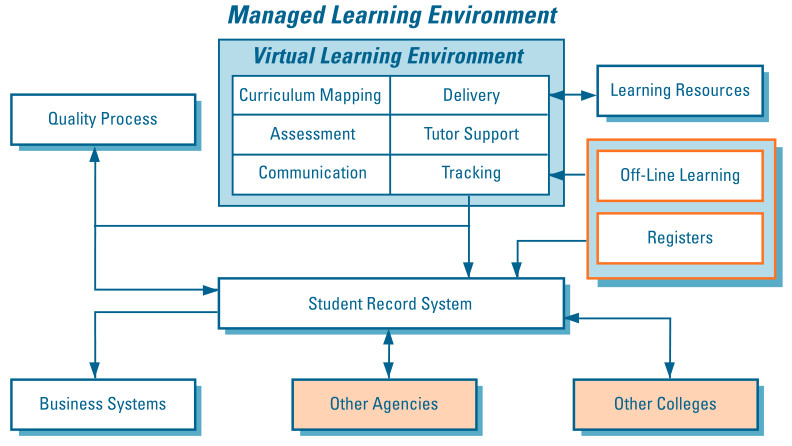
\includegraphics[scale=0.4]{../figures/MLE.png} 		
	\caption{\label{Figure: MLE} Components of an \gls{MLE} \citep{mle}} 	
\end{figure}

This project focuses on the assessment system in the \gls{VLE}.

\section{Types of Assessment}
\label{Section: Types of Assessment}

In education, summative (or `assessment of learning' \citep{digiassess}) and formative (or `assessment for learning' \citep{digiassess}) assessments are often used to provide different types of feedback to students and show their level of progression and competence. The method of assessment will depend on the perspective of the assessor (see \autoref{Table: Perspectives on Learning}).

\begin{longtable}{|L{0.185}|L{0.25}|L{0.21}|L{0.25}|}
\caption[Perspectives on learning]{\label{Table: Perspectives on Learning} Perspectives on learning and approaches to assessment and feedback (from \citep{digiassess})} \\
\hline \textbf{Perspective on learning} & \textbf{Assumption} & \textbf{Assessment} & \textbf{Feedback} \\ \hhline{|=|=|=|=|} \endhead
\multicolumn{4}{c}{Continues on the next page...} \endfoot
\endlastfoot
\textbf{Associative} & \textbf{Learning as acquiring competence} \newline Learners acquire knowledge by building associations between different concepts. \newline Learners gain skills by building progressively complex actions from component skills. & Concepts and competencies frequently assessed at micro level and in combination through macro-level tasks. & - Expert feedback focusing on weaknesses in skills and conceptual understanding \newline - Interactive environments for knowledge and skills acquisition \eoline
\textbf{Constructivist} & \textbf{Learning as achieving understanding} \newline Learners actively construct ideas by building and testing hypotheses. & Assessment by means of experimentation, discovery and inquiry-based tasks. & - Self-generated feedback arising from reflection and self-assessment \newline -Interactive discovery environments with opportunities for self-testing \eoline
\textbf{Social constructivist} & \textbf{Learning as achieving understanding} \newline Learners actively construct new ideas through collaborative activities and dialogue. & Collaborative and cooperative tasks involving shared expression of ideas. \newline Participation by learners in the design of assessment tasks. & - Peer feedback arising from collaborative activities and dialogue \newline -Interactive environments that support sharing and peer feedback \eoline
\textbf{Situative} & \textbf{Learning as social practice} \newline Learners develop their identities through participation in specific communities of practice. & Holistic assessment in authentic or simulated professional contexts. \newline Participation in social practices of inquiry and assessment. & - Socially produced feedback from multiple sources \newline - Feedback derived from authentic real-life tasks \newline - Interactive environments that simulate professional practice \eoline
\end{longtable}

Summative assessment is used when achievement levels need to be reported against a set of published criteria, often as an end of course evaluation. As all students are evaluated against the same criteria their results can be combined to form league tables etc. \citep{assessmentTypes}. These assessments are generally high-stakes so ``those being assessed are likely to do all they can to conceal ignorance and suggest competence" \citep{knight2001briefing}. The feedback from such assessments is usually a mark, often given as a level of achievement or competence rather than specific details on how the assessment could have been completed more successfully.

Formative assessment is not strictly based on criteria but takes into account students' progress and effort \citep{assessmentTypes}. The marks given for formative assessments may use the performance of students from several occurrences. These performances may be inconsistent but these differences in behaviour can be used as a diagnostic to locate where problems are \citep{assessmentTypes}. Formative assessment must be student centred as its two main aims are to get students to recognise the gap between the understanding level they have achieved and what is required, and for the students to take action to close this gap \citep{usesOfAssessment}. To identify the gap immediate feedback on how to improve is required \citep{eps265979} and the disclosure of concepts that are difficult needs to be encouraged \citep{knight2001briefing} to be able to provide effective feedback. 

The choice to use formative or summative assessment will depend on the purpose of the test. If a level of competence is required then summative assessment would be more appropriate. However a test to highlight the areas that the students are struggling with would be better as a formative assessment.

\section{eAssessment}
An \gls{eAssessment} (also known as \gls{CAidA}, \gls{CAssA}, \gls{CBA}) is the process of making, viewing and scoring assessments using a computer. In this report these processes will be carried out by several tools - the ``\gls{authoring}" will be responsible for creating the questions and assembling the test and the ``\gls{delivery}" will be responsible for displaying and scoring the assessments. These tools must be interoperable, meaning they must use data formats that are compatible with each other.

This project focuses on the use of quizzes and polls within videos as a means of assessment.

\subsection{Quiz Definition Standards}
\label{Subsection:Quiz Definition Standards}
In order to store and display the questions in an \gls{eAssessment}, a schema for the questions must be defined. The only formally defined standard found was IMS Global's \gls{QTI} specification\footnote{\url{http://www.imsglobal.org/question/\#version2.1} [Last Accessed: 24 Nov 14]}. Some other quiz (wiki-like) definitions were found including Moodle's General Import Format Technology (GIFT)\footnote{\url{https://docs.moodle.org/28/en/GIFT_format} [Last Accessed: 24 Nov 14]} and Aiken formats\footnote{\url{https://docs.moodle.org/23/en/Aiken_format} [Last Accessed: 24 Nov 14]}.

GIFT is a question mark up by Moodle\footnote{\url{https://moodle.org} [Last Accessed: 24 Nov 14]} and allows the use of a text editor to create questions in some simple formats. There is a strict compliance to specific syntax required and for complex questions it is no longer intuitive \citep{failQTI}. Aiken is another mark up that is designed to be more easily human-readable, again it has strict syntax that must be adhered to or the imports to Moodle would fail.

\gls{QTI} is an interoperability standard for \glspl{eAssessment}. The specification overview \citep{qtiOverview} splits the \gls{eAssessment} system into five systems: authoring tool, item bank, test construction tool, assessment delivery system and learning system (see \autoref{Figure: QTI components}).

\begin{figure}[h]
	\centering 
		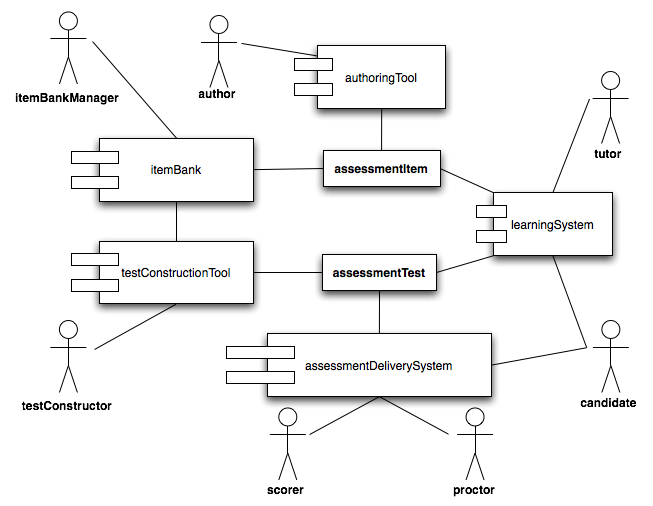
\includegraphics[scale=0.6]{../figures/componentsQTI.png} 		
	\caption{\label{Figure: QTI components} QTI components diagram \citep{qtiOverview}} 	
\end{figure}

In the \gls{QTI} definition the authoring tool is used to create individual questions. However many systems combine this with the Item Bank and Test Construction Tool. For this report ``\gls{authoring}" refers to this combination and, as such, an authoring tool is used to create whole quizzes.

\todo{Does this need a [X] reference like gary mentioned?}
\Citeauthor{wikieassessment} (\citeyear{wikieassessment}) state:
\begin{quote}
The major promise of QTI is that by introduction of common format developers can concentrate on developing innovative tools, whereas teachers can focus on defining new and groundbreaking methods of how to apply those tools in an online environment.
\end{quote}

It is a very complex specification with many ambiguous or optional elements. The complexity of the specification increases the likelihood for errors in the implementation as it opens up opportunities for developers to interpret the specification in different ways \citep{failQTI}. This means the intent of the original author may be lost.

\gls{QTI} v2.1 was finalised in 2012 \citep{qtiOverview} but up to this point the standard was not widely used \citep{eps265979} as there were several fundamental flaws in the standard. When the v2.1 draft was withdrawn in 2009 Rib Abel (IMS GLC CEO) was quoted as saying (on v2.0) ``it’s deficiencies are well known and IMS does not recommend implementation of it [\dots] the only version of QTI that is fully endorsed by IMS GLC is v1.2.1"\footnote{\url{http://lists.ucles.org.uk/public/ims-qti/2009-March/001463.html} [Last accessed: 25 Nov 14]}. This standard gave definitions in natural language. These could often be long-winded and ambiguous, making the standard difficult to implement \citep{failQTI, Sclater2007}.

\gls{QTI} v2.1 defines 18 types of interaction (question, answers and response patterns) \citep{qtiImplementation}:
\begin{multicols}{3}
\begin{enumerate}
\item Choice
\item Order
\item Associate
\item Match
\item Gap match
\item Inline choice
\item Text entry
\item Extended text
\item Hot text
\item Hotspot
\item Select point
\item Graphic order
\item Graphic associate
\item Graphic gap match
\item Position object
\item Slider
\item Drawing
\item Upload file
\end{enumerate}
\end{multicols}

In addition, assessment items can have template and/or adaptive behaviour giving 72 options for each item's type. 

Template items have variables in the questions and answers. These are set as the question is viewed. This allows similar questions to be defined using the same assessment item (e.g. changing the numbers in a maths problem).

Adaptive items are scored over a series of questions. Different questions are displayed based on the answer given for the previous question(s) in the sequence. This branching behaviour is defined by setting the \lstinline!adaptive! attribute to \lstinline!true!. 

\subsection{Usage of Video in eAssessment}
\label{Subsection:Usage of Video in eAssessment}
Video is often used as a medium to convey educational material as it appeals to different learning styles. When video is streamed there is a lack of interactivity and user control \citep{eps267281, DeBoer}. To involve the user more, interactive elements must be added. \todo{Reference style? see above todo question} \Citeauthor{eps267281} found that 75\% of users agreed or strongly agreed that interactive video had enhanced their learning experience but at the time of the paper (\citeyear{eps267281}) they could find no evidence of interactive video being used as a learning tool. There are now some interactive videos being used as a learning tool \citep{nadia} but not widely in \glspl{MLE}.

Interactive videos have often been implemented in Flash \citep{interactiveVideo, eps267281}. This is no longer supported on many devices in favour of HTML5 technologies \citep{flashDead}. The interactivity in HTML5 video players is generally implemented using clickable areas or pop ups \citep{interactiveHTML5}. HTML5 video players do not require an external plug-in to run so will be browser independent \citep{epifania2011design, interactiveHTML5} however some standards are not implemented in all browsers. 

Interactive videos including polls and quizzes is one method that could be used to give a formative assessment. This would give immediate, meaningful feedback, a key feature of formative assessment \citep{eps265979}. Having the questions integrated into the video allows the appropriate sections to be automatically re-watched, encouraging immediate action on feedback. 

\subsubsection{Accessibility and Usability}
\label{Subsubsection:Accessibility and Usability}
To allow interoperability between the \gls{eAssessment} systems the \gls{QTI} specification involves both the model and the view of the data \citep{wikieassessment} making accessibility difficult to add in later. This means many systems that comply with the \gls{QTI} specification are inaccessible.

\gls{eAssessment} systems require an \gls{authoring} that is easily understood by people who do not have an in depth technical knowledge (e.g. teachers). Often authoring tools that implement the \gls{QTI} standard are too technical for this \citep{wikieassessment}. These tools need to improve their accessibility and usability, keeping the time commitments for users reasonable \citep{eps271236, eps265979} or they will not be used.

\todo{Fix reference style} \cite{nadia} did a check for accessibility and other features on existing applications that use video e-quizzes and found that none of them were accessible from a keyboard (see \autoref{Table: Existing Video e-Quizzes}). This means that they do not conform to the \gls{UAAG} of the \gls{WAI} \citep{uaag}. Further research showed that Moodle also uses a video player to display content that is completely inaccessible to a user only using a keyboard\footnote{\url{https://tracker.moodle.org/browse/MDL-36081} [Last Accessed: 24 Nov 14]}. 

\todo{This paragraph seems to just be a random comment, probably needs to be tied into our project a bit more}Using a HTML5 video player keyboard accessibility is easy to implement as the player controls are HTML5 elements. These elements can individually be allowed to gain focus and have a tab order implemented to give full keyboard navigation of the player.

\begin{longtable}{|L{0.17}|L{0.135}|L{0.135}|L{0.13}|L{0.15}|L{0.11}|}
\caption[Existing Video e-Quizzes]{\label{Table: Existing Video e-Quizzes} A comparison between existing systems with interactive video e-quizzes (from \citep{nadia})} \\
\hline \textbf{Criteria} & \textbf{Adobe Captivate} & \textbf{Camtasia Studio} & \textbf{Edpuzzle} & \textbf{Educannon} & \textbf{Hapyak}  \\ \hhline{|=|=|=|=|=|=|} \endhead
\multicolumn{6}{c}{Continues on the next page...} \endfoot
\endlastfoot
\textbf{Version} & Desktop & Desktop & Web & Web & Web \eoline
\textbf{HTML5 support} & \CheckmarkBold & None & \CheckmarkBold & \CheckmarkBold & \CheckmarkBold \eoline
\textbf{Replay function} & None & \CheckmarkBold & None & None & None \eoline
\textbf{Flash fallback} & \CheckmarkBold & \CheckmarkBold & \CheckmarkBold & \CheckmarkBold & \CheckmarkBold \eoline
\textbf{Accessibility} & None & None & None & None & None \eoline
\textbf{Overlay support} & None & \CheckmarkBold & None & None & \CheckmarkBold \eoline
\end{longtable}

There are many ways of conveying content in a video and none of the methods alone will generally convey the whole message. Most video searches stay on a whole resource level as there is a lack of semantic interlinking \citep{eps273063}. Annotation systems such as Synote\footnote{\url{http://synote.org/synote/} [Last Accessed: 24 Nov 14]} aim to make videos accessible by adding transcripts and other annotations to them. The videos being annotated may not be owned by the annotator.

\subsection*{Conclusion}
\label{Subsection: eAssessment Conclusion}
It was decided not to use the \gls{QTI} standard due to the complexity and difficulty of implementing accessibility. The time constraint on this project would mean that more time would be spent on ensuring compliance with \gls{QTI} than implementing the tools.

A HTML5 video player will be used to play the videos. This will enable mobile devices that no longer support flash to play the interactive videos. The HTML5 control elements will simplify the implementation of keyboard accessibility.

The focus of this project would be on creating accessible quiz authoring and delivery tools.

\section{Analytics}
\label{Section:Analytics}
Meaningful analysis of video data is difficult as you need to know the content of the video to understand why the sections may have been of interest to the user \citep{videoLectures}. \Citeauthor{videoLectures} proposes that extra features can be added to the video to aid automatic analysis to be useful, including: multiple (parallel) cognitive channels, semantic marking, transcripts and annotations. Video viewing styles have been researched for non-interactive videos (streaming) and in general four main styles were identified \citep{DeBoer}:
\begin{itemize}
\item \textbf{Linear} - A student watches a video in one-pass (uninterruptedly) from the beginning to the end
\item \textbf{Elaboration} - A student watches a video again after finishing the first time in one-pass
\item \textbf{Maintenance rehearsal} - A student watches parts of a video repeatedly
\item \textbf{Zapping} - A student skips through the instructional video at intervals of relatively short viewing times
\end{itemize}

With the growing popularity of \glspl{MOOC} analysis of video tutorials has been important to increase their usage. \Citeauthor{engagement} \todo{Fix reference style} made several findings such as:
\begin{itemize}
\item Shorter videos are much more engaging
\item Khan-style tablet drawing tutorials are more engaging than PowerPoint slides or code screencast
\item Students engage differently with lecture and tutorial videos
\end{itemize}
These findings would also apply to video quizzes but as the quizzes add a new element to the material the interactions will be different and there will be many more things that could be learned from studying their usage patterns.

Currently there is little research into viewing styles of interactive videos with quizzes and polls in them as there are few tools to capture the necessary data. \Citeauthor{videoAnalytics} created an analytics tool that showed the quizzes separately to the video\footnote{\url{http://www.socialskip.org/home} [Last accessed: 1 Dec 14]} to create graphs of video usage patterns. They used the YouTube player to collect the usage data and Google Drive to include quizzes. They chose to display this information in graphs of video time vs frequency.
%% ----------------------------------------------------------------
%% OverallApproach.tex
%% ---------------------------------------------------------------- 
\chapter{Overall Approach} 
\label{Chapter:Overall Approach}

\section{3rd Party Libraries}
Several pieces of third party software formed the core functionality for our project to build on.

\subsection{AngularJS}
\label{Section:AngularJS}
AngularJS\footnote{\url{https://angularjs.org/}} is a JavaScript Framework that extends HTML attributes. It is an open source library made by Google.

The underlying design pattern used by AngularJS is client side Model-View-Controller (MVC). This is where the data (model), appearance (view) and actions that can be applied (controller) are separated out to make encapsulation and code reuse easier. 

The library allows custom HTML tags and attributes to be created using directives. Directives allow the user to specify the behaviour of specific elements they have created.

One of Angular's most prominent features is its use of two-way binding. This synchronises the views with the data held in the model. This is especially useful when dealing with dynamic content as when extra content is added it is automatically shown in the view.

\subsection{Videogular}
\label{Section:Videogular}
Videogular\footnote{\url{https://github.com/2fdevs/videogular}}\footnote{\url{https://github.com/2fdevs/bower-videogular-controls}} provides a HTML5 video player for AngularJS.

\subsection{UIBootstrap}
\label{Section:UIBootstrap}
UIBootstrap\footnote{\url{http://angular-ui.github.io/bootstrap/}} will be used to give a consistent appearance to all of the user interfaces within the project. It provides Bootstrap components written in AngularJS.

\subsection{Flask}
\label{Section:Flask}
Flask\footnote{\url{http://flask.pocoo.org/}} is a python web application framework that allows you to create web applications with simple routing patterns in python. We have decided to use this for all of our back end web services.

\section{Modular Webserver Approach}
\label{Section:Modular Approach}
It is important for our project to be easily integrated into other projects, specifically we are looking to have it integrated into the latest version of Synote (see section X?). To accomplish this we have designed the back end systems to ensure they can be run without depending on any other modules. All of the functionality will be able to be accessed by REST calls.

By abstracting all calls to using REST this means that other services will be able to interact with out back end services in a language independent way. To facilitate this we have had to ensure that all REST responses are returned with a Cross-Origin header. This allows servers who are not on the same machine to be able to communicate with the REST service.

These features will allow an external application to be able to run the webserver separately and communicate with our server side code. This ensures that the only dependency added by those that use our code will be that they need to be able to make REST calls.
%% ----------------------------------------------------------------
%% ProjectManagement.tex
%% ---------------------------------------------------------------- 
\chapter{Project Management} 
\label{Chapter: Project Management}

\section{Initiation} 
\label{Section:Initiation}

Although as a whole the group had never worked together in the past, some existing close working relationships existed due to previous group coursework. As such it was easy to form the group and begin producing impressive results.

\subsection{Skills Audit} 
\label{Section:Skills Audit}

Many of the strengths and weaknesses of the group members were clear from previous work, but a skills audit was undertaken to ensure that the group as a whole was competent to complete both the coursework and the project without fault.

To begin with a requirement analysis was performed to determine exactly what skills were needed. These split into three very clear general subsections: project management and leadership, from the perspective of both the coursework and the project; technical; and communication. 

Next an audit of each teams members skills were performed, the results of which can be found in \autoref{Chapter:Skills Audit Results}. From these an analysis of the groups total skills was determined and the groups weaknesses could be found.

\section{Task and Work Management} 
\label{Section:Task and Work Management}

This project was run using a Scrum project management approach. This involved having weekly sprints where each person completed a number of tasks, either alone or collaborating with others. Planning meetings were held at the start of each sprint where the issues in the backlog were discussed. They were prioritised and given a point value which related to how much time and effort the issue would take to resolve. The highest priority issues were then assigned. Each person had a maximum capacity of points for each week. Additionally retrospectives were held just prior to the planning meetings to discuss the previous sprints and the way in which the project management was being carried out.

This structure meant that planning and the monitoring of the project happened formally on a sprint by sprint basis. But throughout the project we were careful to adapt when needed, and not be too constrained by the Scrum model. At points in the project where progress presentations had to be created, practised and presented we ran ``mini-sprints'' both for the presentation, and work to be completed in the remainder of the week.

\todo{SCRUM roles - vauge jist of what was done and not complete}

\todo{Burndown charts and other statistics}

%http://tex.stackexchange.com/questions/86114/github-like-punchcard-with-the-help-of-pgfplots
\begin{figure}
  \makebox[\textwidth][c]{
\begin{tikzpicture}                                             %1
        \begin{axis}[                                               %2
                grid=major,                                         %3
                point meta=explicit,
                xmin=-1,
                xmax=24,
                xlabel=Hours,                                       %7
                scatter/@pre marker code/.code={
                    \pgfmathparse{                                  %12
                        \pgfplotspointmetatransformed/1000*8}   %13
                    \def\markopts{                                  %14
                        mark=*,                                     %15
                        color=black,                     %16
                        fill=black,                      %17
                        mark size=\pgfmathresult}                   %18
                    \expandafter\scope\expandafter[\markopts]},
                scatter/@post marker code/.code={
                    \endscope},
                symbolic y coords={Sun,Sat,Fri,Thu,Wed,Tue,Mon},
                xtick={0,...,23},
                x=0.6cm,
                y=0.9cm]
            \addplot[only marks,scatter]
                table[x index=0, y index=1, meta index=2] {punchcard.dat};
        \end{axis}
\end{tikzpicture}
  }%
  \caption{Caption}
  \label{fig:key}
\end{figure}



To allow for collaborative work a GitHub organisation\footnote{\url{https://github.com/soton-ecs-2014-gdp-12/}} was used. This acted as our central source code repository for not only all directly related work, but also work on presentations and reports. Separate repositories for each area of the project are located here for ease of access. Using GitHub made it easier to interact with other open source projects, and all our pull requests and releases were directed from here. 

GitHub also provided an issue management system on a repository by repository basis. This allowed us to track conversations around different bugs and enhancements as the project progressed.
The group used \url{http://www.waffle.io} to manage the issues backlog from a project wide perspective as this would interface directly with GitHub.

\section{Communication} 
\label{Section:Communication}

The project had a reasonably large number of stakeholders that needed to be managed and kept informed. Each stakeholder required different levels of communication via different methods.

The most important stakeholder was the client, Professor Mike Wald. Weekly meeting were organised, minutes of which can be found in Appendix BLAH, and emails were used for urgent issues. 
\todo{Appendix of minutes}
\todo{Managing client - signoff, etc}
Another important stakeholder was Yunjia Li. He attend the weekly meetings as much as possible so as to ensure his future interests in the framework were protected. He was also contactable via email when needed.

2fdev, the Videogular development team, were communicated with via Gitter\footnote{\url{https://gitter.im/2fdevs/videogular}}, an online chat system added onto GitHub. They had an ongoing interest with the framework due to its role of advertising the Videogular project.  There advice and code proved invaluable throughout the project.

\todo{Shameem stakeholder/team member/client discuss}




%% ----------------------------------------------------------------
%% VideoPlayer.tex
%% ---------------------------------------------------------------- 
\chapter{Video Player} 
\label{Chapter:Video Player}

\chapterpreamble{Specific improvements to \gls{Videogular} were made up three main sections, accessibility, compatibility and scrub bar plugin creation. Each were conducted independently and the open source contributions accepted readily back into the main \gls{Videogular} project.

The main goals for this part of the project were to:
\begin{itemize}
\item investigate \gls{Videogular} to allow for its use within the new version of Synote
\item improve the accessibility of \gls{Videogular} to allow for its use by users with less than normal interface  devices
\item ensure that \gls{Videogular} was as compatible on as many devices as possible
\item add the ability to mark locations on the scrub bar
\item produce a plugin to allow the display of statistical data along the scrub bar
\end{itemize}}

\section{Accessibility} 
\label{Section:Accessibility}
\gls{Videogular} has the option to display HTML controls for the video player, replacing the browser's built-in controls. However, when the project began there was no way for the user to access these controls without a mouse. The main problem was that the controls did not identify themselves as interactive elements, and so could not be `focused' (selected with the tab key). This also prevented them from being picked up by a screen reader.

Some online video players allow the player as a whole to be focused, and then controlled with various keyboard shortcuts. The problem with this method is that accessibility aids, such as screen readers, will not have information on these controls, and so users of those technologies will have to be instructed. It is also not accessible to users of a clicker, who can only press one key and so require individually focusable controls.

\subsection{Design and Implementation} 
Instead, the controls were made individually focusable by using semantic markup where possible, and \gls{ARIA} attributes otherwise. When a control is in focus, a visual indicator is displayed to highlight it. Buttons can then be pressed using the space bar (\fref{Figure:Accessibility/Screenshots/Button}); the scrub bar can be moved using the left and right arrow keys (\fref{Figure:Accessibility/Screenshots/ScrubBar}); and the volume can be adjusted using the up and down arrow keys when the mute button is focused (\fref{Figure:Accessibility/Screenshots/Volume}).

\begin{figure}
	\begin{subfigure}[]{\textwidth}
		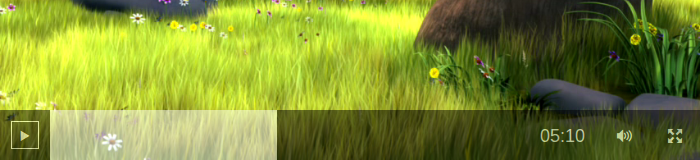
\includegraphics[width=\textwidth]{accessibility/button}
		\caption{The play button when focused. In this state, pressing the space bar plays or pauses the video.}
		\label{Figure:Accessibility/Screenshots/Button}
	\end{subfigure}
	\begin{subfigure}[]{\textwidth}
		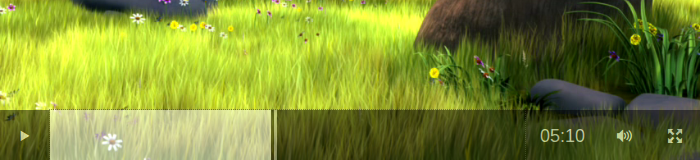
\includegraphics[width=\textwidth]{accessibility/scrub-bar}
		\caption{The scrub bar when focused. In this state, pressing the left or right arrow keys skips backwards or forwards in the video.}
		\label{Figure:Accessibility/Screenshots/ScrubBar}
	\end{subfigure}
	\begin{subfigure}[]{\textwidth}
		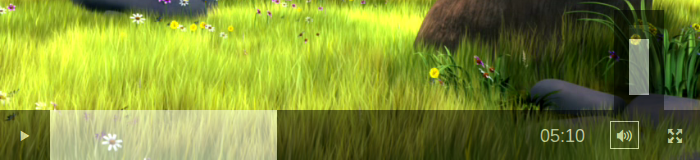
\includegraphics[width=\textwidth]{accessibility/volume}
		\caption{The mute button and volume control when the mute button is focused. In this state, pressing the space bar toggles mute, and the up and down arrow keys change the volume.}
		\label{Figure:Accessibility/Screenshots/Volume}
	\end{subfigure}
	\caption{Screenshots of the accessibility improvements made to Videogular's HTML controls.}
	\label{Figure:Accessibility/Screenshots}
\end{figure}

\subsection{Conclusions} 
This solution is not completely clicker-accessible, but could be made so by introducing buttons to skip forwards or backwards, and to raise or lower the volume. It is a significant improvement on the original state, as keyboard users can now use the player. The improvements were submitted to the \gls{Videogular} project\footnote{\url{https://github.com/2fdevs/videogular/pull/108}}, and are now part of \gls{Videogular} 0.6.1.


\section{Compatibility} 
\label{Section:Compatibility}

One of the main focuses of this part of the project was to make sure the application was compatible with a range of platforms, operating systems and devices. The first challenge was to ensure that the player and overlay displayed correctly at a variety of resolutions and screen/window sizes. 

Apple iPhones provided a problem as iOS forced the video to be played in fullscreen mode. This is a design choice and there is no way to play the video inline, directives to do this are ignored by the browser.

This meant that the video paused at the correct time but as the video is in the native player the overlay was not visible unless the player is quit. There is no way of notifying the user that this needs to be done. A possible solution involves telling the user to quit out of the video when it is paused so they may answer the question. However this is not very user friendly. iOS software on Apple tablets however does not have this limitation and the video will play inline correctly as the device is large enough.

Android phones correctly interpret the inline directive and will properly play this. This ensures that the overlay is correctly applied and usable. This has been the primary focus on testing on mobile devices as it represents a very large portion of the market.

The overlay which displays the questions that the user is asked appears above the video and obstructs the view of the video. Placing the overlay in the middle of the screen requires a large amount of \gls{CSS} to correctly locate it on the screen for mobile and smaller sized devices. There are still some issues with the popup location on some mobile devices because the browser reports one screen size and uses another. Until these devices are compliant with the specification it is time consuming to write code to fix each individual case.

The best user experience with this application is using it on a desktop that has an updated browser. This will definitely work and display as intended. As the screen size of the device gets smaller the user experience is significantly reduced as the video and poll overlay will be much smaller than recommended. To support a number of browsers and operating systems a range of video formats are supplied to the \gls{Videogular} plugin so that the browser may pick one that can be played.

\section{Scrub Bar Extensions} 
\label{Section:Scrub Bar Extensions}

\gls{Videogular} has been designed and implemented in such a way as to allow for directive-based plugins to be developed to extend its functionality. When using the \gls{Videogular} Controls (vgControls) the native browser controls are replaced with an HTML based interface. It is this interface we have improved the accessibility of, and it is the scrub bar within this interface we have created plugins for.

The team behind \gls{Videogular}, 2fdev, are actively seeking members of the community to develop new plugins for their system, and as such are willing to discuss future plugins and their architectural design.

\subsection{Videogular Cuepoints - vgCuepoints}
\label{Subsection:vgCuepoints}
\gls{Videogular} Cuepoints is a \gls{Videogular} plugin for displaying `cuepoints', marks on the scrub bar which can be positioned at a particular time. For example, cuepoints could be used to indicate the start of a section in the video, or a time when a pop-up will appear.

\subsubsection{Design and Implementation}


\subsection{Videogular Heatmaps - vgHeatmap}
\gls{Videogular} Heatmaps is a \gls{Videogular} plugin for giving areas of the scrub bar different colours. In our examples this is used to give a visual representation of the number of times each section of the video has been watched.

\subsubsection{Design and Implementation}
An early design decision was to use \gls{CSS} to colour the sections as this would allow different colours to be specified (see \cref{Req:Use of colour}). This also would allow developers to develop their own colour schemes with meanings if they desired.

Sections and colours can be specified in a \texttt{config} object which is given as a parameter when the heat map is used. 

The schema for defining the configuration parameters was made consistent with vgCuepoints (see \autoref{Subsection:vgCuepoints}) to improve usability.

One problem found during implementation was that the heat map cannot be displayed before the video has begun playing. This is due to \gls{Videogular} not setting the video length variable until it begins playing, thus this variable cannot be used to calculate the widths of the sections until it is set. This was accepted as the colouring does not have any context for a user until they have watched the video.

An extra option that was added for improved accessibility was the ability to label each heat map section with the frequency. Extra hidden text was added so that a screen reader user could still access all the data shown in the heat map. 

\section{Conclusions} 
\todo{Overarching video player conclusion}
%% ----------------------------------------------------------------
%% Overlay.tex
%% ---------------------------------------------------------------- 
\chapter{Overlay - vgQuestions} \label{Chapter:Overlay}

\todo{I am not sure what the following list is trying to convey, should it be
removed?}
The overlay was built up in stages:
\begin{enumerate}
\item Getting an overlay to appear at a set time
\item Adding in question types
\item Allowing custom question sets to be used
\item Returning the answers to a server
\end{enumerate}

\section{Annotations}
\label{Section:Annotations}

One of the main issues to address early on was how to represent the quiz and
poll questions. The QTI (Question \& Test Interoperability) specification was
investigated, but was found to be complicated and incomplete \todo{What does
incomplete mean here?} for the project needs. It was decided to design a new
format for representing the data and logic that is used for a particular
application of videogular-questions.

This new format separates the front end of the library (responsible for
interacting with the DOM), from the data and logic regarding the questions by
means of a message passing interface. This is achieved in a rigorous way in the
browser by means of a WebWorker. This is a sandboxed separate thread that run
in the background the webpage. They run independently of standard user-space
scripts.  More can be found out about their use within this project in Section
BLAH.

Using JavaScript, rather than a pure data representation (e.g. JSON or XML)
allows for the use of JavaScript to provide the logic. This makes it extremely
flexible and concise, and the isolation provided by the WebWorker mitigates
many security concerns with having an application that executes data given as
input as code.

\begin{lstlisting}[language=javascript]
importScripts("../questions-worker.js");

loadAnnotations({
  "first-annotation": {
    // the time that this annotation will show up
    // (in seconds from the start of the video)
    time: 1,
    items: [
      {
        id: "first-question",
        type: "single",
        question: "What is the moon made of?",
        options: [
          {
            name: "cheese"
          },
          {
            name: "cheeese"
          },
          {
            name: "cheeeeeese"
          }
        ],
        correctAnswer: "cheese"
      },
      {
        id: "check-question",
        type: "single",
        question: "Answer incorrect, do you want to review the video",
        options: [
          {
            name: "Yes"
          },
          {
            name: "No"
          }
        ],
        action: function(questions, video) {
          if (questions.get("check-question").response === "Yes") {
            video.setTime(0);
          }
        },
        condition: function(questions) {
          return questions.get("first-question").isNotCorrect();
        }
      }
    ]
  }
});
\end{lstlisting}

Every item in an annotation can have an action and condition function. The
action function is called when a item finishes. The action function is given
the state of the annotations, such that it can make decisions and then affect
the state of the video accordingly. For example, in the above example, this is
used to only have the "skip back" question show, if the answer given to the
previous question is incorrect.

The condition function is called to determine if the respective item will show.
By default, when an annotation is shown, each item is shown in sequence.
However, if an item has a condition function, this is evaluated, and the item
only shown if the condition function returns true. If the condition function
returns false, the item is skipped. This functionality is used in the above
example to have the video skip back if the user wants it to.


An early decision was to define the difference between a poll and a quiz
question. It was decided that a poll is a type of quiz question that does not
have a correct answer.

Initially basic question types (single choice, multiple choice and scale
questions) were focused on. A variety of visualisations was implemented
including check boxes, radio buttons and sliding scales. Validation was needed
to ensure that the specified minimum and maximum limits were followed.

By having a standard schema that uses JavaScript functions it was possible to
write template functions that could be outputted from the authoring tool and
read by the overlay correctly.

\section{Front End}
\label{Section:Front end}

The appearance of the overlay depends on the question type to be shown. The
layout of these different types was carefully considered for accessibility and
ease of use. Mockups were made and user studies were done in collaboration with
a third year project student.

A set of example css files are supplied with the project that layout the
questions according to the feedback received. Developers using any part of the
project can use these styles as is, or modify/develop their own.

\section{Back End}
\label{Section:Back end}

\subsection{Web Workers}
\label{Subsection:WebWorkers}

Web workers give a good way of running (sandboxed) background scripts that are
computationally intensive. They are a way of multithreading - allowing multiple
scripts to run simultaneously, avoiding the problem of unresponsive pages due
to long running scripts. This is done by using message passing.

For example, when an answer is submitted by the user this would sent a message
to the webworker containing the answer. The webworker can then process this
information without affecting the responsiveness of the page. Once the
processing is complete the webworker can send a message back to the page to
tell it what to do next.

\begin{sequencediagram}
  \newthread[white]{c}{Front End}
  \newinst[4]{s}{WebWorker}

  \mess{s}{annotations}{c}

  \stepcounter{seqlevel}
  \begin{call}
    {c}{annotationStart}
    {s}{showQuestion}
  \end{call}

  \stepcounter{seqlevel}
  \begin{call}
    {c}{questionResult}
    {s}{showQuestion}
  \end{call}

  \stepcounter{seqlevel}
  \begin{call}
    {c}{questionResult}
    {s}{endAnnotation}
  \end{call}
\end{sequencediagram}

The above diagram illustrates the messages that could pass between the web
worker, and the front end when the above example is used. Initially, the worker
sends a annotationStart message. This contains the times which annotations will
occur.

When the first time is reached, the front end sends a annotationStart
message to the worker, containing the id of that annotation. The worker then
replies with a showQuestion message, containing the contents of the first
question. Note that here, the functions are not sent to the front end, just the
JSON representation of the question is sent.

When the user responds to the question, that response is send to the worker in
a questionResult message. In this case, the user responded incorrectly,
therefore, when the web worker evalutated the condition on the second question,
it evaluated to false. This meant that the worker replied with another
showQuestion message.

Once the user responds to the second question, the response is again sent to
the web worker. In this case, this was the final question in the annotation, so
the worker responds with an endAnnotation message.

\section{Interaction with Analytics}
\label{Section:vgQuestions Analytics}

Since we were writing a series of plugins we wanted to ensure that no one
plugin required another to be used effectively. Instead of a custom method of
communicating between two or many possible plugins we decided to use the
publish/subscribe model to communicate with the vgAnalytics plugin.

Using the angular broadcast system we could publish events on channels which
then would be received by anyone who subscribed to that channel.

The below code snippet shows how we communicated to the vgAnalytics plugin.

\begin{lstlisting}[language=javascript]
$rootScope.$broadcast('analytics','show_question', data);
\end{lstlisting}

Here we broadcast to the ``analytics'' channel an event with the name
``show\_question'' with the content of the data variable.

The vgAnalytics plugin listens to the ``analytics'' channel and they will
receives all messages published to this. Therefore vgQuestions can publish
information which will be received by the vgAnalytics plugin. If it has not
been instantiated then these messages will not cause any errors which is one of
the important factors in picking a communication method between the various
plugins.

By using the publish/subscribe model we can design the plugin so that if they
are both being used they will work together but have no dependencies on each
other. This allows any of our plugins to be used together or separately as the
user wishs.

%% ----------------------------------------------------------------
%% Authoring.tex
%% ---------------------------------------------------------------- 
\chapter{Authoring Tool} 
\label{Chapter:Authoring Tool}

\chapterpreamble{The authoring tool section details the motivation for creating a tool that is able to produce the \gls{DF} used by the \gls{vgQuestions} plugin. One of the key features was that the tool should be accessible and is able to describe the wide range of features the \gls{vgQuestions} plugin supports.}

\section{Introduction}
\label{Section:Authoring_Introduction}

An accessible \gls{authoring} was required to allow users to create their own question sets. Within the authoring tool users can create polls and quizzes and overlay them at chosen locations in a video. This avoided the necessity for users of the framework to learn the JavaScript quiz format, thus significantly reducing the technical barrier to entry. 

One key consideration during the implementation of the authoring tool was accessibility. The \gls{WCAG} 2.0 guidelines were kept in mind at all times and adhered to as much as possible.

Care has been taken to ensure that the authoring tool can be easily used within other AngularJS projects, and thorough documentation has been provided to ease this process.

\section{Design} 
\label{Section:Authoring_Design}

Within the authoring tool users have the ability to create questions sets within a video. There could be any number of questions in a set and these could be of many different types. A range of options are given to modify the functionality of each question so as allow the user to create exactly what they need.

At any point the user can preview the quiz they have created on the inbuilt video player. Once they are satisfied with the quiz they can export it for use with videogular-questions externally from the tool.

It was decided to use Bootstrap\footnote{\url{https://github.com/twbs/bootstrap/}} to give a consistent appearance to all of the user interfaces components within the project. This is a HTML, \gls{CSS}, and JavaScript framework for developing webpages.

As an Angular framework is used, any additional functionality is required to be written as directives and controllers. UIBootstrap\footnote{\url{http://angular-ui.github.io/bootstrap/}} provides some Bootstrap components written in \gls{AngularJS}. This provides some of the components required. 

Wireframes were created using this style so that they could easily be directly coded as static HTML to allow a quick demo to be created. 

Two different approaches were suggested for showing the advanced options for the video. A pop up approach hid these from general view to avoid confusing users with lots of options that may be unnecessary. The other approach was to use the accordion structure as we had for the questions. This would be collapsed by default so the options would still be hidden. This was chosen as it was more consistent with the rest of the tool. Wireframes were created to allow for feedback from users and the customer. They can be found in \autoref{Chapter:Authoring Tool Wireframes}.

\section{Implementation}
\label{Section:Authoring_Implementation}
Once the wireframes were drawn up they could be turned into static HTML. Elements of this webpage were then incrementally given the functionality they required. The main challenge was ascertaining how the functionality fitted in with the \gls{AngularJS} Framework. 

Each section of the page had to have its own directive so that independent behaviours could be achieved. This kept the HTML pages short and readable as the behaviour was dealt with by the JavaScript and the styling dealt with by the \gls{CSS}.

Angular allowed the dynamic nature of the data to define the appearance of the page. Sections could be set to appear only when certain attributes were set using ng-switch statements. This meant one section could potentially show many different elements depending on what was selected elsewhere on the page.

\subsection{Data Bubbling}
\label{Section:Authoring_Data_bubbling}

With the authoring tool we have leveraged the ability to use two way binding and watches with AngularJS. This allows us to template a number of reusable elements such as the time picker and means we don't have to rewrite the class each time we wish to use it. This has reduced the time taken to produce the authoring tool.

The root controller holds the global state of the authoring tool. This global state is updated by the child controllers who each own specific parts of the global model. This bubbling of data up the controllers is the key to how the authoring tool has been built.

The preview and generation features utilise this model in the root controller composed from the bubbled models over the child controllers.

\begin{figure}[h]
	\centering
		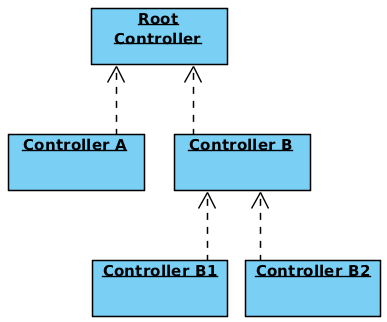
\includegraphics[scale=0.4]{../figures/authoring_tool/controller_bubbling.png} 		
	\caption{\label{Figure: Bubbling model data} Bubbling of model data up controllers} 	
\end{figure}

\autoref{Figure: Bubbling model data} shows the general structure of the controllers and how we have implemented the bubbling up of data. In our implementation we have a large number of controllers and levels to encapsulate the different ways of quiz creation. In this diagram controller A and B will bubble their model data up to the root controller if it changes. If model data in controller B1 or B2 changes, their new model will bubble up to controller B. Controller B will then will then bubble its model combined with the new model data it has received to the root controller.

This bubbling technique works for any number or levels of children provided the model data is correctly bubbled up each layer. It also makes adding new controllers at any point simple as you only need to handle the bubbling of the data up the levels.

Each controller may have one or more children who may or may not hold model data.

\begin{figure}[h]
	\centering
		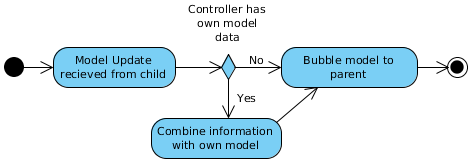
\includegraphics[scale=0.6]{../figures/authoring_tool/bubbling_to_root.png} 		
	\caption{\label{Figure: Bubbling to root} State diagram illustrating decisions when bubbling data to root} 	
\end{figure}

\autoref{Figure: Bubbling to root} demonstrates the decision making process to determine how the controller bubbles the data. Any controller that does not hold important model data will only bubble any information sent to it to the root controller. Any controller that has a model will also bubble its own model and model data received upwards. Therefore the global model is slowly accumulated by bubbling up the data. When it reaches the root controller the global model has been built and is saved for later use.

A controller holding model data stores the state of the controller which is represented by a HTML view. Each view is bound to its specific model using two way data binding. This means when the view is changed by the user the model will be automatically updated.

\begin{figure}[h]
	\centering
		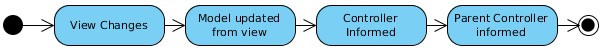
\includegraphics[scale=0.6]{../figures/authoring_tool/two_way_binding.png} 		
	\caption{\label{Figure: Authoring two way binding} Two way binding bubbling method illustrated in an state diagram} 	
\end{figure}

\autoref{Figure: Authoring two way binding} shows the process of the view changing and updating its parent. Each time the model is updated the controller runs any appropriate action to change the display of the view then sends the updated model to its parent. This change is bubbled upwards each level until it reaches the root controller who stores the new data in its global model.

\subsection{Exporting of Data}
\label{Section:Authoring_export_data}

As the user is selecting the options for their quiz, the data will be bubbled up as described in \autoref{Section:Authoring_Data_bubbling}. Once they have finished creating their quiz they will be able to press the export button. When this is pressed the global model is reviewed, and the corresponding \gls{DF} is generated.
\begin{lstlisting}[language=javascript,caption={Base template for authoring tool \gls{DF} generation},label={code:authoringToolTemplate} ]
test
/* jshint worker: true */
"use strict";

importScripts("WORKER_URL");

/* global loadAnnotations */
loadAnnotations(ANNOTATION_DATA);
\end{lstlisting}

First the global options are processed and the basic file is created. This uses a default template which is stored in the authoring tool. The current template used is shown in \autoref{code:authoringToolTemplate}. This has two sections that are replaced with content that are generated in a later stage. These are `WORKER\_URL' and `ANNOTATION\_DATA'. `WORKER\_URL' is currently replaced by the URL as guessed by the authoring tool. This may need to be modified if the vgQuestions plugin has been modified to move the web worker position. `ANNOTATION\_DATA' is replaced with the generated question data that is generated below.

Once the template has been created, each question set is processed. This involves taking all the settings for the question set, storing it the question set format, and then processing and generating JavaScript for each question in the question set.

When generating the JavaScript for each question the question type is used to generate a set of attributes specific to that question type. The attributes generated are as defined in the class diagram \autoref{Figure:questions_class_diagram} and these are added to the question.

\begin{lstlisting}[language=javascript,caption={Base template for a question asking if the viewer wishs to review the video section they answered incorrectly},label={code:authoringToolTemplateRewatchSection} ]
{
	id: "incorrect-QUESTION_ID",
	type: "single",
	question: "Answer incorrect, do you want to review the video",
	options: [
		{
			name: "Yes"
		},
		{
			name: "No"
		}
	],
	action: function(questions, video) {
		var question = questions.get("QUESTION_ID");
		if (question.response !== question.correctAnswer) {
			video.setTime(TIME);
		}
	},
	condition: function(questions) {
		return questions.get("QUESTION_ID").isNotCorrect();
	}
}
\end{lstlisting}

For some questions, there will be a number of different annotation questions added to the question set. One example is when the quiz author has selected that a user may return to a specific point if they fail a question. This will add a question asking the user if they wish to review the section of the video containing the answer to the question. This template is shown in \autoref{code:authoringToolTemplateRewatchSection} and has the variables `QUESTION\_ID' and `TIME' which will be replaced with the data from the question the user has enabled the option on.

Once an individual question has been generated the next question in the question set will be processed.

Once all of the questions in a question set has been processed it will continue onto the next question set.

Some options allow you to add results at the end of the video. These settings are stored up and once the all question sets have been processed this is added onto the end of the `ANNOTATION\_DATA' string.

\begin{lstlisting}[language=javascript,caption={The final \gls{DF} is offered for downloading using a data blob URL},label={code:authoringToolFileDownload} ]
var url = "data:text/json;charset=utf8," + encodeURIComponent(data);
window.open(url, "_blank");
window.focus();
\end{lstlisting}

Once all of these options have been calculated the final template is produced. The template string have their content inserted to generate the finished \gls{DF}. To allow the user to download the file easily we construct a blob url with the code in \autoref{code:authoringToolFileDownload}. Without using a data URL we would require the user to copy the text generated and save it. As this was not a user friendly option so we investigated possible other uses. Offering a file for download was problematic because JavaScript does not have any write permission for files since it is client side. The data blob URL solution provides an acceptable solution by mocking up file URL with data. This may encounter issues with larger files due to the max length permitted in a URL but we have not yet seen these issues occur.

\subsection{Preview tool}

The preview tool works similar to the export tool (\autoref{Section:Authoring_export_data}) by generating the \gls{DF} and creating the blob URL. Once this has been done this is passed to the vgQuestion plugin embedded in the authoring tool which loads up the newly created quiz.

This allows for immediate feedback when creating the quiz and makes it easier to create a quiz for non technical users (\cref{Req:User interface}). Since we have embedded the vgQuestions plugin we will be sure that this will react the same when added to a website using the plugin.

\section{Conclusion}
\label{Section:Authoring_Conclusion}

The tool we have produced allows a user to create the \gls{DF} in the correct format that can be used vgQuestions to display user created quizzes.

\cref{Req:Keyboard accessibility} outlines the importance of accessibility so we have designed the authoring tool to be as accessible as possible. \autoref{Section: Conformance of Authoring Tool} details our conformance to the \gls{WCAG} standards. In \autoref{Section:Testing_Authoring_tool_accessibility} we have ran through a number of testing methods applied to the authoring tool to demonstrate that it is accessible and outlined any further issues.

\autoref{Figure:Authoring_Tool} is an image showing our final user interface. The colour scheme was chosen to be high contrasting to fulfil \cref{Req:Use of colour}. In addition the CSS used to set this colour scheme is in a single place and is easy to change as to a users requirement.

To further decrease the barrier to entry (\cref{Req:User interface}) we used the \gls{Videogular} and \gls{vgQuestions} plugin to allow a preview of the quiz they have created. One of the useful side effects of \cref{Req:Standalone} has meant that it has been easy to integrate \gls{vgQuestions} into the authoring tool.

\begin{figure}[h]
	\centering
		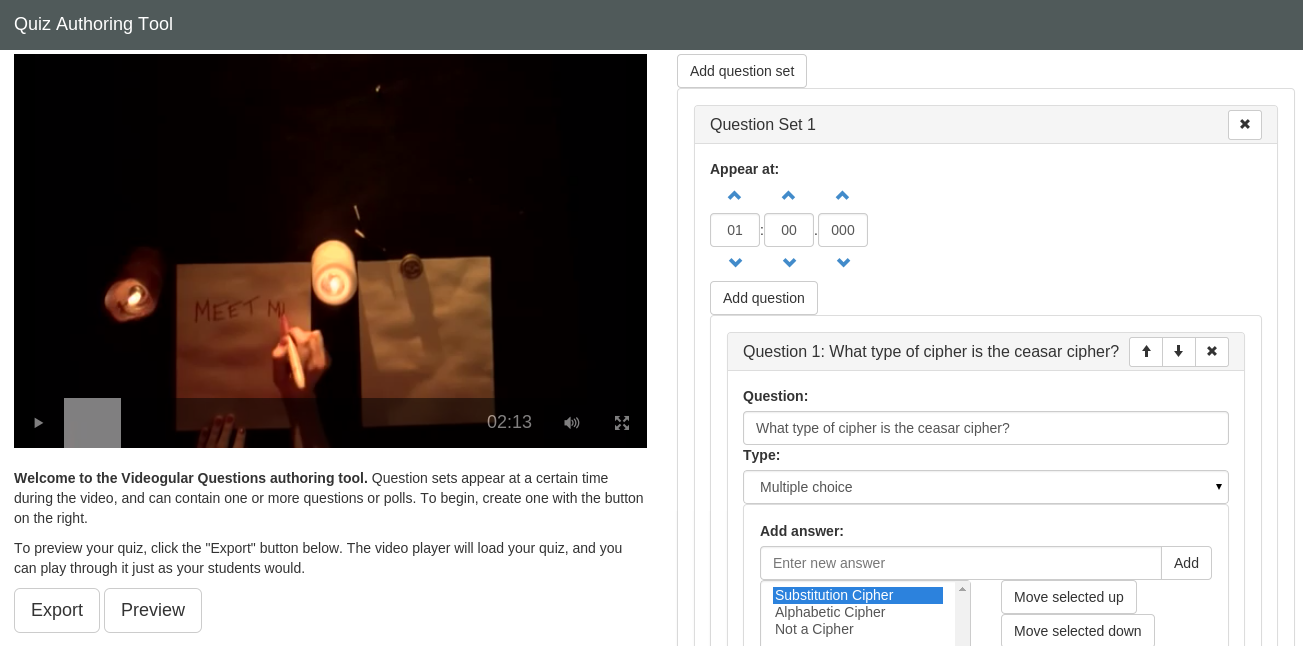
\includegraphics[width=\textwidth]{../figures/authoring_tool_example.png} 		
	\caption{\label{Figure:Authoring_Tool} Image showing the final authoring tool being used} 	
\end{figure}

There may be some more work needed to investigate how large a JavaScript quiz file may be produced when using the data blob URL approach to allow the user to download the file. While no limits problems have occurred during testing this is something that will need to be kept in mind.
%% ----------------------------------------------------------------
%% Analytics.tex
%% ----------------------------------------------------------------

\chapter{Analytics} \label{Chapter: Analytics}

\begin{preamble}
	\preamblequote{I never guess. It is a capital mistake to theorize before one has data. Insensibly one begins to twist facts to suit theories, instead of theories to suit facts.}{Sir Arthur Conan Doyle, Author of Sherlock Holmes stories}
\end{preamble}

\section{Introduction}

One of the main requirements states  that video and question events should be emitted from the Videogular player (\cref{Req:Analytics events}. We decided that instead of putting analytics events directly into the \gls{vgQuestions} plugin we would make a new plugin to handle analytics.

This plugin will monitor how the user uses the videogular video player and the vgQuestions plugin and store events related to this. If a server is configured this will send the users data to a server where it can be aggregated and processed.

\section{Design}

The reason for designing the plugin to be separate from the main vgQuestions plugin is because not all users of the core functionality will also want to perform analytics. This means that for users that are not interested their will be no overhead of collecting the data. This can be important on mobile devices that have smaller processing power available.

In addition, implementing this as a separate plugin means that it is not dependant on any of the other plugins and therefore fulfils \cref{Req:Standalone}.

Since the plugin is the published deliverable it will be used with an external server to capture the data. This will be able to aggregates this and store it in some format. It is configured to post data via \gls{REST} calls (\cref{Req:Server architecture}) to a server defined in the analytics configuration file.

There will be a published \gls{API} to be used with the analytics plugin that will detail all events will be published form the plugin. A well documented API is important (\cref{Req:Documentation}) so that developers can easily create a service that collects and uses the data.

In the event that the server is unable to be contacted it should queue the results until it comes back online. Once a request fails to be sent the plugin should try sending all queued events at an interval until the server comes back online or the application is closed. If the application is closed before the server comes back online the data will be lost.

\subsection{Analytics emitted events}

The Videogular Analytics plugin emits a number of events which can be sent to a Web server for collection. \autoref{Table:analytics_api} describes all events emitted from the analytics plugin.

The plugin is designed so that events can easily be added by sending events to the \pre{analytics} channel. These are automatically collected and prepared for sending to the given Web server.

\begin{tabular}{p{3.2cm} p{6cm} p{4cm}}
\caption{\label{Table:analytics_api}API of the emitted analytics events and their data payload}
\textbf{Event name} & \textbf{Emitted when} & \textbf{Expected Payload} \\
\hline
show\_question & a question is shown to the user & All of the associated question data \\
\hline
end\_question & the annotation being shown has finished & None \\
\hline
show\_results & there are results that will be shown & The results data being shown \\
\hline
submitted\_question & the user submits a question & The chosen question response \\
\hline
skipped\_question & the user skips a question & None \\
\hline
continue\_question & a results page is closed by pressing the continue button & None \\
\hline
play & the video starts to play & The time the video plays from \\
\hline
pause & the video is paused & The time the video pauses at \\
\hline
stop & the video is stopped & The time the video was stopped at \\
\end{tabular}

\section{Implementation}

The plugin itself watches videogular, and triggers events when videogular's state changes. Other plugins can report events by sending a event to angular with the name ``analytics''.

The plugin will then forward all the events to all of the servers. It does this in a standard format that make it easy to process all the events, and just select the ones that are required for the analysis that is being performed.

If the plugin is not in use, then any events reported by other plugins will simply not be processed, as there will be nothing listing for the events called ``analytics''.


%% ----------------------------------------------------------------
%% Testing.tex
%% ---------------------------------------------------------------- 

\chapter{Testing} \label{Chapter: Testing}

\begin{preamble}
Software testing is necessary on projects of all sizes, especially on large projects such as this. To ensure quality throughout the project each part of the framework has been thoroughly tested. This chapter details different testing methodologies along with the results of the tests.
\end{preamble}

\section{Introduction}

During development number of testing methods were used for each section of the project to reflect the different types of module. All sections that have requirements that directly specify features such as \cref{Req:Keyboard accessibility} will have user acceptance tests performed. These tests directly form part of the deliverables report (\cref{App:Deliverable Report}).

A number of sections have a deliverable sign-off table. While working in an agile method a working program that could be presented to the client at any time was kept. This was usually done during the client/supervisor meetings. During final tests number deliverable sign-off tests were created that were used to prove to the customer that the software worked correctly. These were presented in the deliverable report (see \cref{App:Deliverable Report}) that was presented to the client and signed off.

These deliverable sign-off tests were used as manual regression tests. These were used during the final changes and bug fixes to ensure the functionality that the client wished were still present and working correctly.

\section{Tools}

A number and range of different tools have been used during testing to ensure that the quality of the code is to the high standard the customer required. For each repository the types of tests that are applicable were decided and can be implemented to properly test the application.

\subsection{Unit Testing Plan}
\label{Section:Testing_unittesting}

Where possible unit test style tools have been used to automate repeatable types of tests. Anyone working with a repository that has unit tests should follow the following policies:

\begin{itemize}
\item \textbf{Running unit tests after checking out new code} - This is to ensure that all code checked out is currently working. If it does not they are encouraged to look into fixing the problem themselves or determining which commit broke the build and contact the committer to find the reason for this.

\item \textbf{Create unit tests for new functionality} - The unit tests form part of our continuous testing plan with the aim to ensure all code on master branches runs properly. Adding unit tests for new features helps ensure this as others will be able to run them to check your new features are working correctly after other code modifications have been made.

\item \textbf{Run unit tests before committing new code} - As a final check before submitting new code, all unit tests should be run on the repository. This acts as a final confirmation to ensure that no new code has broken old code. This forms part of the regression testing. Any older code that has been broken must be reviewed and fixed to ensure that the master branch runs properly.

\item \textbf{Fix broken unit tests} - When a unit test is identified that it is not working as intended it should be reviewed to see if it is still applicable and ensure that it is modified to work if so. There may be multiple reasons why a unit test has been broken so it may be needed to contact the person who originally broke the unit test to find out what was changed and why.
\end{itemize}

The tools we have used in the testing sections below are described fully in the following subsections.

\subsection{JSHint}

JSHint is a tool for static code analysis of JavaScript, which can detect many instances of bad coding practice in source files before they cause errors. Included in each of our repositories containing JavaScript is a configuration file for JSHint, which enforces use of ECMAScript 5 Strict Mode, and prohibits use of undeclared variables or type coercion. JSHint was run at regularly during the project and any issues it highlighted were fixed. For repositories that had JSHint set up for use it was recommended to run this before committing.

\subsection{Karma}

Karma allows tests to be run in browsers (or headlessly) in an automated manner.  It then also aggregates and displays the results making it easy to see if the tests have passed or failed.

Karma is included within Angular seed (see \autoref{Section:Overall_Testing}), which means it was available from the start. The inclusion in Angular seed was one of the reasons it was used as it is an industry standard for AngularJS.

\subsection{Jasmine}

Jasmine is a testing framework for JavaScript. It has simple syntax and works well with Karma.

Jasmine was also included in Angular seed (see \autoref{Section:Overall_Testing}) and therefore already set up for use.

This has been used as the unit test framework for AngularJS code within the project.

\subsection{Python unittest module}

Python has included in its standard packages, a module called unittest. This module is designed to be similar to the JUnit testing framework for Java and this has been used for all python based projects as a unit test framework.

\subsection{Locust}

Locust\footnote{\url{http://locust.io/}} is a distributed load testing tool that allows you to define a site access pattern. By designing a site access pattern you specify how often sites are visited relative to others and therefore can tailor the access patterns to your likely use case.

This tool has been used as it is able to give percentile data to see statistics on how fast all requests are fulfilled. Many other similar tools only give an average request time which will cause problems when some users are kept waiting for a much longer time. Having access to a full set of statistics allows the running of performance checks and improvement of features so no users are left waiting.

\section{Videogular Questions Example} 
\label{Section:Videogular Questions Example}

The Videogular Questions Example site was written as testing and documentation for how Videogular Questions, Videogular Cuepoints and Example results server could be used. This is helps to fulfil \cref{Req:Documentation} and \cref{Req:Documentation}.

\subsection{Videogular Questions}
\label{Subsection:Videogular Questions in example}

There are several tests written for the \gls{vgQuestions} plugin. These use Jasmine, and can be run in an automated way using Karma.

These tests exercise the web worker component of the \gls{vgQuestions} plugin over the message passing interface. A script is used, which contains messages to send, and expected responses. A test passes if the script runs as expected with no missing or extra messages.

The examples created in the Videogular Questions Example repository use individual or collections of features. These were used in the development of these features, and in the demonstration of these features to the customer.  These examples complement the Jasmine tests, as they exercise the display elements of the plugin.

There was no user experience testing done directly as part of the project, as the client had reservations about user experience testing due to the toolkit style nature of the project. Shameem performed some user experience testing for the Videogular Questions Example site and these were discussed in a meeting with both Shameem and the client \autoref{subsection:Meeting10Nov}. The consensus was that while the results were informative, they were outside the scope of this project.

\subsection{Videogular Cuepoints}
\label{Subsection:Videogular Cuepoints in example}
\gls{Videogular} Cuepoints was integrated into the example site, and configured to mark the times at which pop ups were displayed. The issue where marks could only be displayed once the video began to play (as described in \autoref{Subsection:vgCuepoints}) was the only problem encountered.

\subsection{Example Results Server}
\label{Subsection:Example Results Server in example}

For the example results server there was a small set of functions to test with a small number of possible inputs and a well defined set of responses. This is, therefore, well suited to individual unit tests.

Flask\footnote{\url{http://flask.pocoo.org/}} is a python web application framework that allows you to create web applications with simple routing patterns in Python.

The Flask library had a test client and recommended test skeleton\footnote{\url{http://flask.pocoo.org/docs/0.10/testing/}} which was made use of to run the unit tests. This used the unittest standard python library which meant it was easy to test with but also allowed calling of methods by simulating HTTP requests.

The testing was split into 6 areas to test the main components of the application: cross-origin resource sharing, routing, database setup, voting, getting results and load testing.

\subsubsection{Cross-Origin Resource Sharing tests}

One of the main requirements by the customer was that these units should be able to be accessed via \gls{REST} calls (see \cref{Req:Server architecture}). In addition the requirement stated that there should be no reliance that these servers are on the same host. To ensure that these \gls{REST} calls will not fail cross origin resource sharing headers were implemented as discussed in \autoref{Section:Modular Approach}.

This checks to ensure that the Cross-Origin Resource Sharing (CORS) header is correctly sent in the HTTP reply. If this is not set the web browser will likely reject the loading of the page and the application will fail.

In addition, it ensures that the response is the one expected and not an error state to ensure that the web application is also sending the correct content.

\subsubsection{Routing tests}

The routing tests are to ensure that the application correctly starts and is accessible.

If this fails to load up the testing URL which returns "Hello World!" then it is unlikely to be able to perform some of the more complex functions.

\subsubsection{Database Setup tests}

Before the application can be used it needs have its database set up. This is performed by accessing `/setup'. This set of unit tests test setting up a database and ensure that if this URL is visited twice, it successfully detects that the database is already set up and does not recreate it. 

This is important to ensure that the database is set up correctly and that when setup is visited again data in the database is not lost.

\subsubsection{Voting tests}

These tests try a number of different ways to vote by sending a number of different formats of invalid and valid data to check if the application correctly deals with the data. All return codes and responses are checked to ensure no invalid vote is accepted or valid one rejected.

\subsubsection{Getting results tests}

A number of valid votes are constructed and then sent into the system. Then these are attempted to be retrieved. The returned values are checked to ensure that they have not been corrupted. This submits one and multiple votes to ensure that all votes are correctly collated and returned.

If the ability to vote does not work then this will fail as it relies on being able to put votes into the system.

\subsubsection{Load testing}

For the load testing we have used Locust and have chosen three access patterns to test the example results server:

\begin{itemize}
\item Visiting the root page - This is to determine that the webserver is still responding to basic HTTP requests
\item Voting - This is to test that the voting functionality is still accessible
\item Requesting data - This is to test that the server is still able to return data
\end{itemize}

These three URLs were visited repeatedly by the user clients over a period of time.

\begin{table}
\caption{Time taken for each request to complete in milliseconds while stress testing the example results server}
\begin{tabular}{l c  c c c c c c c c }
\hline 
& & \multicolumn{8}{c}{Percentile} \\
Name & Requests & 50\% & 75\% & 80\% & 90\% & 95\% & 98\% & 99\% & 100\% \\ 
\hline 
GET / & 535 & 5 & 50 & 67 & 110 & 170 & 240 & 360 & 601 \\ 
\hline 
GET /results/*/* & 1599 & 6 & 26 & 46 & 100 & 136 & 233 & 326 & 326 \\ 
\hline 
POST /vote & 1129 & 120 & 150 & 170 & 210 & 250 & 360 & 460 & 638 \\ 
\hline 
Total / Average & 3263 & 32 & 110 & 120 & 160 & 210 & 270 & 400 & 638 \\ 
\hline 
\end{tabular}
\label{Table:stress_testing_results_server}
\end{table}

\autoref{Table:stress_testing_results_server} shows the time taken for a response to be handled and returned.

Here you can see that the time taken for result requests takes less than 6 milliseconds 50\% of the time and all requests were dealt with in at most 326 milliseconds. The voting \gls{REST} point takes slightly longer as it needs to store data to the sqlite database but still took at most 638 milliseconds. All these tests were performed when 50 Locust users were using the website continuously and therefore it was agreed that the performance should scale. This is because one user will only ever make one vote and one results request per question and this tested for 50 users continuously making these requests.

Although this is only an example this ties in with \cref{Req:Scalability} that the results server should perform normally when a lecture room full of people is using it. The testing shows that the application is able to cope with 50 people continuously voting and therefore should be able to cope with a much less strenuous 300 people casting votes over a period of several minutes.

There is also scope to move the back-end database to something that is purely in memory to further increase the speed, as the major factor will be writing the data back to the hard disk.

\subsection{Accessibility}
\label{Subsection: vqe accessibility}

The \gls{Videogular} Questions Example was mostly accessible by the WCAG 2.0 standards (see \autoref{table: vqe conformance}). However the lack of alternatives for the video and the cuepoints using only colour may cause issues for some users.

The lack of captions or signed versions of the videos was down to the videos used so not was an issue with the page overall as it is a proof-of-concept.

A textual alternative was not provided because the idea is to integrate this into Synote which provides a transcript (see \autoref{Section:Synote}). Thus, this feature would be duplicated.

The cuepoints are only conveyed through the changing of colour on the scrub bar. In future extra behaviour could be added to these to make them accessible through other means.

As a proof-of-concept this site showed that it is possible to create an accessible questions overlay when combined with Synote.

\subsection{Deliverable signoff tests}

These tests in \autoref{table:vgQuestions Deliverable signoff tests} were presented to the client as the deliverable items for the Videogular Questions and Videogular Cuepoint plugins.

These tests were ran on the Videogular Questions Example website. This had examples of all types of questions and therefore was used as a deliverable for the customer.

\begin{center}
\begin{longtable}{|L{0.9}|L{0.03}|} 
\caption{\label{table:vgQuestions Deliverable signoff tests}vgQuestions Example Deliverable signoff tests} \\
\hline \textbf{Detail of test} & \rot{\textbf{Pass }}\\ \hline
\endfirsthead
\hline \textbf{Detail of test} & \rot{\textbf{Pass }}\\ \hline \endhead
\multicolumn{2}{c}{Continues on the next page...} \endfoot
\endlastfoot
Single Question provides radio buttons to select at most one answer. & \CheckmarkBold \eoline
Question Multiple provides checkboxes to select one or more results. The min/max values should be shown and \keys{Submit} should be disabled if these requirements are not met. & \CheckmarkBold \eoline
Questions Star should allow you to click on the stars and select one rating. The Min/Max values should be shown and \keys{Submit} should be disabled if these requirements are not met. & \CheckmarkBold \eoline
Questions Text should allow you to enter a textual value before submitting. & \CheckmarkBold \eoline
Question Range should present a slider which allows you to choose a range of values. The min/max values should be shown on the slider. & \CheckmarkBold \eoline
The tabs Single Question, Question Multiple, Question Stars, Question Text, Question Range all should show one demonstration of the specific question type. & \CheckmarkBold \eoline
The poll simple example should show an example poll. & \CheckmarkBold \eoline
Caesar Example should have Videogular Cuepoints enabled so you will be able to see where the questions will be shown. & \CheckmarkBold \eoline
Caesar Example's second question at the end of the example will have a poll to see the results of all those who have answered the question. & \CheckmarkBold \eoline
\end{longtable}
\end{center}

The pass marks show each test was tested by the developers on this project and was successful, and also accepted by the client after review of the deliverable report.


\section{Example Analytics Server}
\label{Subsection:Analytics server in example}

The analytics back-end server receives the \gls{REST} calls from the \gls{Videogular} Analytics plugin and is then able to process them. For this example implementation it was chosen not to store the data but forward it to the front-end. This will demonstrate that the Videogular Analytics plugin is able to make \gls{REST} calls. Storage could be used to collate the information for later recall.

\subsection{Cross-Origin Request testing}

\cref{Req:Standalone} states that each plugin should operate in a standalone manner. It needed to be ensure that the example server and analytics plugin works correctly when performing cross origin requests. To permit this on the example server testing code has been included to permit all cross origin requests, see \autoref{code:analyticsCrossOrigin}.

\begin{lstlisting}[language=javascript,caption={Code showing appending Cross Origin headers to all responses}, label={code:analyticsCrossOrigin}]
app.all('*', function(req, res, next) {
	res.header("Access-Control-Allow-Origin", "*");
	res.header("Access-Control-Allow-Headers",
	           "Origin, X-Requested-With, Content-Type, Accept");
	next();
});
\end{lstlisting}

To test that the analytics worked cross-domain the analytics example site and the Videogular Analytics plugin were set up on two different testing servers. This was able to correctly pass data between the two and therefore passed cross-origin testing.

\subsection{Reloading processed data}
\label{Section:reloading processed data}

The back-end acted as a testing platform for the front-end. A large set of data was recorded from the Videogular Analytics plugin and saved to allow for repeated testing of the same pieces of data. The back-end plugin has a tool to specify a data file that has already been processed to be loaded.

Any front-end client connecting to the back-end \gls{Videogular} Analytics server will be sent all events in the loaded piece of data. This allows the front-end website to be quickly tested with a set of data that encompasses all features of the \gls{Videogular} Analytics plugin. This data set allows comparison between a known valid set of data and data that \gls{Videogular} Analytics creates allowing you to easily identify issues that occur.

This helps to faster identify cases where \gls{Videogular} Analytics is not conforming to the \gls{API} standard.

\section{Example Analytics Front-End}

The example analytics front-end loads up events from the \gls{Videogular} Analytics plugin. These events are obtained by a websocket to example analytics server. In the current model the example analytics server acts as an intermediary between this and the \gls{Videogular} Analytics plugin that can serve additional events as described in \autoref{Section:reloading processed data}.

This front-end tests the \gls{Videogular} Analytics plugin to ensure that the data received is not missing or corrupting events. This is done by loading the data into different formats and processing it. The data processing assumes a number of standard data elements expected from the Videogular Analytics based on the \gls{API} (\autoref{Table:analytics_api}).

\subsection{Videogular Heatmaps}
\label{Subsubsection:Videogular Heatmaps in example}
%Heatmap, user stories, run through

One of the analytics used in the example site is the \gls{Videogular} Heatmap. When running an instance of \gls{Videogular} Questions Example this can be used to dynamically update the heat map in the example analytics page (see \autoref{Figure: Heat map display}).

\begin{figure}[h]
	\centering
		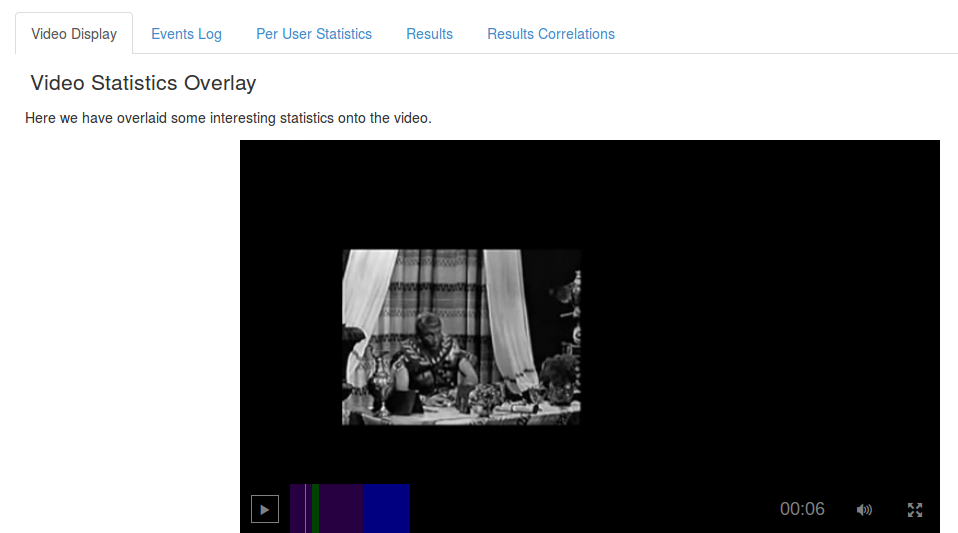
\includegraphics[scale=0.4]{../figures/heatmapDisplay.png}
	\caption{\label{Figure: Heat map display} The heat map has dynamically updated}
\end{figure}

This is used to test that the \gls{Videogular} Analytics plugin is able to properly export the timing data. The processing on the client side matches up start and end marks. These marks shown in \autoref{Figure:Analytics time periods} are then further processed to produce the data that the analytics can use.

If these are not able to be processed then this indicates an issue with the events being sent from the \gls{Videogular} Analytics plugin. If they are able to be sent but the heat map does not display then there is an issue with the heat map.

Running this against the predefined data is used as a regression test for \gls{Videogular} Heatmap to ensure it is working correctly.

By running an instance of the Videogular Questions Example site and voting with the analytics we perform end-to-end testing as this data is passed through a number of our plugins to reach the Analytics front-end to be loaded by the \gls{Videogular} Heatmap plugin.

\begin{figure}[h]
	\centering
		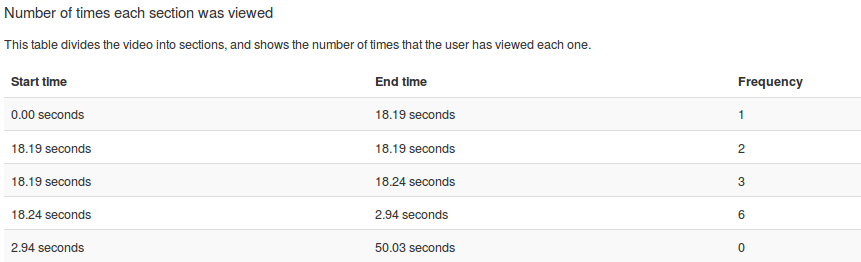
\includegraphics[scale=0.4]{../figures/analytics_time_periods.png}
	\caption{\label{Figure:Analytics time periods} Analytics events after being processed into viewer time periods}
\end{figure}

The added feature of displaying the frequencies was also tested. These displayed well and matched the frequencies represented by the colours used. A screen reader could still access the data as it was declared in hidden text.

\subsection{Videogular Analytics integration with Videogular Questions}

To test integration with \gls{vgQuestions} we have included a set of dynamic graphs that update as events about question results are sent. \autoref{Figure:Analytics Question Graphs} shows an example of the results of questions that have been sent from the plugin.

\begin{figure}[h]
	\centering
		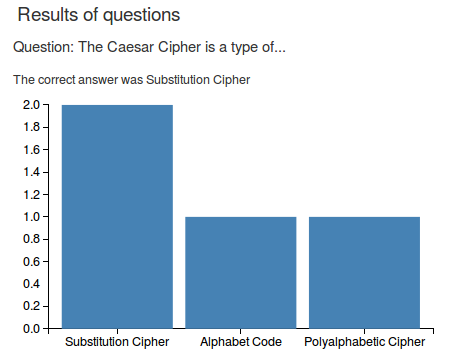
\includegraphics[scale=0.8]{../figures/analytics_graphs.png}
	\caption{\label{Figure:Analytics Question Graphs} Graph showing results of questions sent from Videogular Analytics}
\end{figure}

If the question data is not being received this means that the \gls{Videogular} Analytics plugin has not been able to properly access the \gls{vgQuestions} events. This test was used as a regression test to ensure that the Videogular Analytics plugin is correctly accessing all published analytics events and forwarding them to the \gls{REST} server.

\subsection{Accessibility}

The example analytics site generally conformed to the \gls{WCAG} 2.0 standards (see \autoref{table: va conformance}). The non-conformances found were a lack of alternatives for the video and graphs.

The video issues were the same as for the Videogular Questions Example site (see \autoref{Subsection: vqe accessibility}). However the cuepoints were not used. The heat maps had a textual option that could be displayed which gave additional methods for conveying the information.

Using graphs has created many accessibility issues for visually impaired or cognitively impaired users as the data is not described in text. This would be an important consideration for any developer using our plugins in their own site. As a proof-of-concept the example site purely shows that graphs could be used as a method of automatically producing a visual representation of the data.

\subsection{Deliverable signoff tests}

The tests in table \autoref{table:vgAnalytics Deliverable signoff tests} were presented to the client as the deliverable items for the example analytics tool.

These tests were ran on the analytics tool example using preloaded data so that we had a repeatable set of data that was always valid.

\begin{center}
\begin{longtable}{|L{0.9}|L{0.03}|} 
\caption{\label{table:vgAnalytics Deliverable signoff tests}vgAnalytics Deliverable signoff tests} \\
\hline \textbf{Detail of test} & \rot{\textbf{Pass }}\\ \hline
\endfirsthead
\hline \textbf{Detail of test} & \rot{\textbf{Pass }}\\ \hline \endhead
\multicolumn{2}{c}{Continues on the next page...} \endfoot
\endlastfoot
All events are listed at the top of the events log page, including the type and details of the events & \CheckmarkBold \eoline
The sections that the users have watched are correctly calculated and shown at the bottom & \CheckmarkBold \eoline
Watched video segments are calculated correctly and show how many times all users have viewed a section. & \CheckmarkBold \eoline
The results page shows the user responses. & \CheckmarkBold \eoline
The results page also shows correct answers and whether users rewatched sections. & \CheckmarkBold \eoline
The ``\% watched by correct answers'' and ``Time watched by correct answers'' graphs show two ways you could represent the data in a different way. & \XSolidBrush \eoline
\end{longtable}
\end{center}

Here the final requirement was queried by the customer. The example graphs shown did not have an vertical axis. This was fixed by adding an axis after the customer meeting however during the meeting this did not affect signoff since it was an example of possible graphs that could be created.

\section{Authoring Tool}

The authoring tool is primary deliverable as it is the only item that is designed as a tool and not as a proof-of-concept example site deliverable. Therefore the primary types of testing are deliverable signoff tests and accessibility testing.

\subsection{Accessibility}
\label{Section:Testing_Authoring_tool_accessibility}

The authoring tool was found to be generally accessible conforming to most of the \gls{WCAG} 2.0 standards (see \autoref{table: authoring tool conformance}). The areas that were lacking were providing textual alternatives and error checking.

There were no alternatives provided for the video. However as this would be used with Synote transcripts could be used from there. In future, support for extra accessibility features such as transcripts, captions or signed versions could be included in the authoring tool.

In creating the questions there is no help provided for error checking. This is because it was decided not to narrow the options available to the users. In the occurrences where errors are identified these are generally highlighted by surrounding the component with a red border. More information on how the system would be used would be required in order to create helpful error messages.

Two keyboard accessibility issues were found, both of which were due to browser bugs. The first was that Google Chrome and Chromium did not allow multiple items to be selected in a \texttt{\textless select multiple\textgreater} element using only the keyboard. During the course of the project, a fix was made to Google Chrome and Chromium which allowed multiple \textit{adjacent} items to be selected with the keyboard \citep{ChromiumMultipleSelectBug}, which is an improvement but still not a complete fix.

The second keyboard accessibility issue was that collapsible section headings caused ``focus loops'' in Mozilla Firefox, where pressing the Tab key from the last button on the heading caused the focus to move back to the heading itself, preventing the user from focussing any content after the heading. This was reported on the Mozilla bug tracker \citep{FirefoxFocusLoopBug} (see \cref{App:Firefox Bug Report}), where another user pointed out that the HTML causing the bug was invalid. The HTML was rewritten to be valid, which fixed the issue.

Another issue found was in the use of the \texttt{\textless select\textgreater} element as the colour of highlighted options is not editable in the \gls{CSS}. To solve this issue the elements would all need rewriting to take a completely different structure to allow the \gls{CSS} to modify the colours used.

Accessibility in the authoring tool was good but there are improvements that could be made in future including adding support for accessibility features such as subtitles, providing error correction support and rewriting the \texttt{\textless select\textgreater} elements to allow editing of colours.

\subsection{Deliverable signoff tests}

The tests in \autoref{table:Authoring tool Deliverable signoff tests} were presented to the client as the deliverable items for the authoring tool.

\begin{center}
\begin{longtable}{|L{0.9}|L{0.03}|}
\caption{\label{table:Authoring tool Deliverable signoff tests}Authoring tool Deliverable signoff tests} \\
\hline \textbf{Detail of test} & \rot{\textbf{Pass }}\\ \hline
\endfirsthead
\hline \textbf{Detail of test} & \rot{\textbf{Pass }}\\ \hline \endhead
\multicolumn{2}{c}{Continues on the next page...} \endfoot
\endlastfoot
Pressing \keys{Export} will provide you with a \gls{DF} which can be used. & \CheckmarkBold \eoline
Pressing \keys{Preview} will reset the video back to the start, load the questions into the preview, and begin playing & \CheckmarkBold \eoline
All 5 question types are implemented and, as suggested, the Single choice question (with radio buttons) is merged with the Multiple choice question. & \CheckmarkBold \eoline
A question set is able to be added at a specific time. & \CheckmarkBold \eoline
Once a single question has been added the \keys{Preview} button is used to ensure this is shown properly & \CheckmarkBold \eoline
Each question type is tested along with common options and displays as expected. & \CheckmarkBold \eoline
Skipping is tested for one question and works as expected. & \CheckmarkBold \eoline
When checked, the record button sends the poll data to the poll server. & \CheckmarkBold \eoline
A full walkthrough is attempted, all question types are able to be added and previewing, and exporting works & \CheckmarkBold \eoline
\end{longtable}
\end{center}

The pass marks show each test was tested by us and was successful, and also accepted by the client after review of the deliverable report.

\section{Conclusions}

Working in an agile manner meant that each week work was presented to the client. This meant that the primary types of testing are ensuring functionality works through integration tests and the final deliverable reports. The example websites have been created to demonstrate that the plugin works and to allow testing of them in the environment they are planned to be used in.

Some repositories have been tested using a unit testing strategy(\autoref{Section:Testing_unittesting}) which is focussed on ensuring that regression tests are ran and detection of errors before committing code. For these repositories the master branch should always build and function correctly. This has allowed meetings with the client to always demonstrate working projects while we are at any stage of development.

The analytics front-end server is an example of our integration testing. Here Videogular, Videogular Analytics, and Videogular Heatmap is used to demonstrate a number of statistics about how a user is using the interface. We have tests for each of these modules but identified a number of issues that occurred after linking these plugins together. Videogular Questions, Videogular Analytics, and results server have been tested in this manner using the Videogular Examples website.

In server applications that require a fast response load testing has been performed to ensure that performance degradation would not affect a users experience. This has been shown (\autoref{Table:stress_testing_results_server}) to cause any user to have high latency and suggestions have been made to improve it if needed.

These tests have demonstrated to the client that this has been thoroughly tested and they have signed off the deliverable report(\cref{App:Deliverable Report}) presented to them. The documentation provided also includes recommended practices for continued work to satisfy \cref{Req:Documentation}.
%% ----------------------------------------------------------------
%% FutureWork.tex
%% ---------------------------------------------------------------- 
\chapter{Future work} \label{Chapter: Future Work}

\begin{preamble}
This framework is very much just the beginning, there are a number of interesting improvements that can be made to enhance and extend the project. This chapter details a number of these potential improvements.
\end{preamble}

\section{Introduction}


\section{Integration with Synote}

The most important part of our project is ensuring that the work we have done is easily integrated into Synote.

Therefore during the process we have been in communication with the current developer of Synote to ensure that the work we are doing will be able to be used.

One key requirement was that the work we are doing should be able to stand alone and not require any additional Synote framework but that Synote should be able to communicate with these pieces of work easily (see \cref{Req:Standalone}).

To ensure this all, our services use an open standard to communicate using either \gls{REST} calls, with an associated documentation of each call and how it can be used, or protocols such as web sockets. These services can be run as small webservers which will allow Synote to communicate with them easily. In addition since these are standalone we have been able to pick the best language for the associated service. This has decreased the complexity of our services which should reduce the time needed to learn how the software works in order to continue our work.

The core of the project uses \gls{AngularJS} and the \gls{Videogular} player as this was recommended as the latest version of Synote will be written in Angular. All of the plugins were written for the \gls{Videogular} player and therefore will be able to be easily integrated into the primary Synote codebase. The plugins are the only part that will be integrated into Synote directly and therefore were best suited to be written in Angular. The other services will communicate with Synote and therefore did not need to be written in Angular.

\section{Additional Video Players}

Since our plugins are built upon the \gls{Videogular} system we have not been concerned with how the video is played. The base \gls{Videogular} system plays the common video formats.

To further expand our system we could look at fixing the \gls{Videogular} YouTube Plugin\footnote{\url{https://github.com/NamPNQ/bower-videogular-youtube}}. This would allow users to specify a youtube video to use for the quiz and removes the problems with getting all formats of video for all browsers.

\section{Video Encoding}

\todo{Talk about how we could produce something that removes this requirement}

\section{Mobile Interfaces}

Creating interfaces that work well with mobile interfaces is a difficult task and therefore we have only spent the time to ensure that our basic examples work on most mobile devices.

Further work would be concerned with getting the plugin to work on all devices as iPhones have shown to have significant issues with playing video and overlaying content (see \autoref{Section:Compatibility}).

\section{Second Screen}

A previous project \todo{cite} worked on the possibility of creating a second screening application that worked with Synote. This allowed you to have two views of Synote and display different data on a second screen. This screen would usually be a mobile device for audience members \todo{is this true?}.

If we had time to continue our work we would look into extending the plugin that we have developed to have a "second screen" option for users. This would allow users to turn their mobile device into a second screen for our popups to allow them to answer the questions on their device.

This would also allow a user to take advantage of additional lecture features such as subtitling. Another project is currently being ran to get in lecture subtitles and this could be a feature added as one of our plugins.

\section{Angular 2}

At the 2014 ng-europe conference during a talk about the future development of Angular details about the 2.0 release were given. It is slated for an early 2016 release, with Angular 1.x receiving bug fixes for anther 2 years.

Currently it seems that Angular 2.0 is a complete rewrite of the Angular ecosystem and is only related to Angular 1.x by name. Upon its release applications wishing to stay upto date will need to be rewritten from scratch. As this project is currently built around Videogular, it would first need to be updated and rewritten. This framework's main customer, Synote, is currently in development and as such is using Angular 1.x. 

As such there is potential future work for investigating Angular 2.0 upon its final release. At that time much more information regarding potential upgrade paths would exist.

\section{Cuepoints and Heatmap accessibility}
Currently the only way of getting information from the \gls{Videogular} Cuepoints is through the use of colour. \gls{Videogular} Heatmaps also has the option to include the frequency as text. Although the colours are customisable these plugins are not very accessible. An improvement that could be made in future is to have information available when the marked section is in focus (on hover and when it is playing) that gives the details used by the plugin. For example an area of a heat map could display the number of times the section has been viewed, and the start and end times of the section.

\section{Authoring Tool Accessibility}
The authoring tool accessibility could be improved by adding support for accessibility features such as captions and transcripts. This would aid the improvement of the accessibility of the content when using it in the overlaid video player.

The elements used to create dropdowns and multiple select boxes could also be rewritten to allow the editing of colours in \gls{CSS}.



\section{Conclusions}
%% ----------------------------------------------------------------
%% Conclusions.tex
%% ---------------------------------------------------------------- 
\chapter{Conclusions} \label{Chapter: Conclusions}
It works.

\section{Future work}

Future work.

\subsection{Integration with Synote}

The most important part of our project is ensuring that the work we have done is easily integrated into Synote.

Therefore during the process we have been in communication with the current developer of Synote to ensure that the work we are doing will be able to be used.

One key requirement was that the work we are doing should be able to stand alone and not require any additional Synote framework but that Synote should be able to communicate with these pieces of work easily.

To ensure this all our services use an open standard to communicate using either REST calls, with an associated documentation of each call and how it can be used, or protocols such as web sockets. These services can be run as small webservers which will allow Synote to communicate with them easily. In addition since these are standalone we have been able to pick the best language for the associated service. This has decreased the complexity of our services which should reduce the time needed to learn how the software works in order to continue our work.

The core of the project uses AngularJS and the Videogular player as this was recommended as the latest version of Synote will be written in Angular. All of the plugins were written for the Videogular player and therefore will be able to be easily integrated into the primary Synote codebase. The plugins are the only part that will be integrated into Synote directly and therefore were best suited to be written in Angular. The other services will communicate with Synote and therefore did not need to be written in Angular.

\subsection{Mobile Interfaces - Second Screening}

A previous project [cite] worked on the possibility of creating a second screening application that worked with Synote. This allowed you to have two views of Synote and display different data on a second screen. This screen would usually be a mobile device for audience members [is this true?].

Creating interfaces that work well with mobile interfaces is a difficult task and therefore we have only spent the time to ensure that our basic examples work on mobile devices.

If we had time to continue our work we would look into extending the plugin that we have developed to have a "second screen" option for users. This would allow users to turn their mobile device into a second screen for our popups to allow them to answer the questions on their device. Further work would be concerned with getting the plugin to work on all devices as iPhones have shown to have significant issues with playing video and overlaying content (see section \ref{Section:Compatibility}).

This would also allow a user to take advantage of additional lecture features such as subtitling. Another project is currently being ran to get in lecture subtitles and this could be a feature added as one of our plugins.

\newpage
\bibliographystyle{ecs}
\bibliography{ECS}

\newpage
\phantomsection
\markboth{GLOSSARY}{Glossary}
\printglossary
%TC:ignore
\appendix
%% ----------------------------------------------------------------
%% AppendixProjectManagement.tex
%% ---------------------------------------------------------------- 
\chapter{Skills Audit Results} \label{App:Skills Audit Results}

\begin{preamble}
	An appendix detailing the skills audits that were performed.
	\preamblequote{Debugging is twice as hard as writing the code in the first place. Therefore, if you write the code as cleverly as possible, you are, by definition, not smart enough to debug it.}{Brian W. Kernighan}
\end{preamble}

\section{Skills Audit Matrices} 
\label{Section:Skills Audit Matrices}
A skills audit of the group members was performed and skills audit matrices was produced for all tasks relevant to the project.

Below acronyms for each group member are used in the tables. Each acronym relates to a below member of the group:

\begin{itemize}
\item S - Samuel Bennett
\item H - Harry Cutts
\item CB - Christopher Baines
\item CH - Christopher Hewett
\item M - Maria Lynch
\end{itemize}

\subsection{Project Management} 
\begin{tabular}{ l || l | l | l | l | l || l}
  Task & S & H & CB & CH & M & Average \\ \hline
  Planning & 5  &  3  &  5  &  4  &  5  &  4.4 \\ 
  Progress tracking &  3  &  4  &  5  &  4  &  4  &  4.0 \\
  Time management &  5  &  4  &  5  &  4  &  4  &  4.4 \\
  Contingency planning &  4  &  4  &  5  &  5  &  5  &  4.6 \\
\end{tabular}

\subsection{Technical} 
\begin{tabular}{ l || l | l | l | l | l || l}
  Task & S & H & CB & CH & M & Average \\ \hline
  Technical Research &  4  &  4  &  4  &  5  &  5  &  4.4 \\
  Analysis &  5  &  4  &  4  &  5  &  5  &  4.6 \\
  Architecture Design &  3  &  5  &  4  &  5  &  4  &  4.2 \\
  API Design &  3  &  5  &  4  &  4  &  4  &  4.0 \\
  HCI / Interface Design &  4  &  4  &  4  &  5  &  5  &  4.4 \\
  Implementation \\
   - Client Side &  5  &  4  &  4  &  4  &  5  &  4.4 \\
   - Server Side &  4  &  5  &  5  &  5  &  4  &  4.6 \\
  Evaluation &  5  &  4  &  4  &  4  &  5  &  4.4 \\
\end{tabular}
%Implementation
%	Client Side
%		HTML
%		CSS
%		Javascript
%			AngualrJS
%	Server Side
%		Python
%			Flask
%		Javascript
%			Node

\subsection{Communication} 
\begin{tabular}{ l || l | l | l | l | l || l}
  Task & S & H & CB & CH & M & Average \\ \hline
  Technical Writing\\ 
   - Software Documentation &  4  &  5  &  4  &  5  &  5  &  4.6 \\
   - Report &  5  &  4  &  5  &  4  &  5  &  4.6 \\
  Academic Research &  5  &  4  &  4  &  5  &  5  &  4.6 \\
  Presentation &  5  &  5  &  4  &  4  &  4  &  4.4 \\
  Critical and comparative evaluation &  4  &  5  &  3  &  4  &  5  &  4.2 \\
  Reflection &  4  &  4  &  3  &  5  &  4  &  4.0 \\
\end{tabular}
%% ----------------------------------------------------------------
%% AppendixDeployment.tex
%% ---------------------------------------------------------------- 
\chapter{Deployment of Webservers} \label{App:Deployment of Webservers}

\begin{preamble}
An appendix detailing how each of the tools can be deployed to a website.
	\preamblequote{Intuitive design is how we give the user new superpowers.}{Jared Spool, Web Site Usability: A Designer's Guide}
\end{preamble}

\section{Introduction}

This is divided into the different types of Web server applications we have used. Different Web technologies have been used based on their strengths on what was needed to be produced.

Each repository has a section in the \lstinline|README.md| file detailing how to set up and install the tool. The individual guides have been reproduced below.

\section{Deployment of all projects}

To deploy many of these projects they require you to run \lstinline|npm install| which will also run \lstinline|bower install|. The specific requirements for each application is defined in the \lstinline|README.md| file in each repository.

\section{Deployment of Flask Applications} \label{Section:Deployment Flask Applications}

The only Flask application is the results server therefore this guide is customised to deploy the results server.

To deploy the poll server using Apache first you need to clone the repository.

Then the Apache \lstinline|httpd.conf| file needs to be configured by adding the following entry somewhere in the file:

\begin{lstlisting}[caption={Apache configuration}, label={code:apacheConfig_flask}]
<VirtualHost <hostname>:80>
	ServerName <hostname>
	WSGIDaemonProcess results_server user=<user> group=<group> threads=5
	WSGIScriptAlias / /<location>/results_server.wsgi
	ErrorLog logs/results_server-error_log
	CustomLog logs/results_server-access_log common

	<Directory <location>>
		WSGIProcessGroup results_server
		WSGIApplicationGroup %{GLOBAL}
		Order deny,allow
		Allow from all
	</Directory>
</VirtualHost>
\end{lstlisting}

Parameters needing changes:

\begin{itemize}
\item \textless hostname\textgreater is the hostname of the server. e.g. \lstinline|website.domain.net|
\item \textless location\textgreater is the location of the source code on the server. e.g. /var/www/results\_server/
\item \textless user\textgreater is the user you want the script to run under, by default Apache
\item \textless group\textgreater is the group you want the script to run under, by default Apache
\item The \lstinline|ErrorLog| and \lstinline|CustomLog| parameters can be changed to any location

\end{itemize}

\section{Deployment of Node.js servers} \label{Section:Deployment of Node.js servers}

The only Node.js application is the example analytics backend therefore this guide is customised to deploy this.

Apache cannot directly run Node.js webservices therefore it needs to be ran by node itself.

This can be run by using \lstinline|npm start| which will run the Node server. This needs to be running on the server all the time you want the server to be accessible.
A web search will return details of how to turn a Node.js webserver into a service however it can just be run from the command line using screen or a similar program.

You can configure Apache to proxy any connections to the Node server. This is how we suggest integrating an Apache server with Node.

To do this mod\_proxy needs to be installed, web searches will find guides to install this for your chosen operating system.

Then the Apache \lstinline|httpd.conf| file needs to be configured by adding the following entry somewhere in the file:

\begin{lstlisting}[caption={Apache configuration}, label={code:apacheConfig_nodejs}]
<VirtualHost <hostname>:80>
	ServerName <hostname>
	ErrorLog logs/analytics-error_log
	CustomLog logs/analytics-access_log common

	ProxyRequests off
	
	<Proxy *>
		Order deny,allow
		Allow from all
	</Proxy>

	<Location />
		ProxyPass <analytics address>
		ProxyPassReverse <analytics address>
	</Location>
</VirtualHost>
\end{lstlisting}

Parameters needing changes:

\begin{itemize}
\item \textless hostname\textgreater is the hostname of the server. e.g. hostname.domain.com
\item \textless analytics address\textgreater is the URL for the analytics server. This is displayed when npm start is run. by default this is `http://localhost:5001/`
\item The \lstinline|ErrorLog| and \lstinline|CustomLog| parameters can be changed to any location
\end{itemize}

\section{Deployment of AngularJs Files} \label{Section:Deployment of AngularJs Files}

The authoring tool and \gls{Videogular} Questions example repositories are both written in AngularJS.

AngularJS files are JavaScript and therefore can be run on a normal Apache webserver.

To install these repositories you must clone the repository to a location served by Apache and then install the dependencies by running \lstinline|npm install|

Once this has been performed the application will be able to be used.
%% ----------------------------------------------------------------
%% AppendixAccessibilityStandards.tex
%% ---------------------------------------------------------------- 
\chapter{Accessibility Standards} 
\label{Chapter:Accessibility Standards}
Both of our example user interfaces were tested against the \gls{WCAG} 2.0 Standards\footnote{\url{http://www.w3.org/TR/WCAG20/} (Accessed: 15 Jan 15)} to check for accessibility.

\section{Videogular Questions Example}
\label{Section: Conformance of Videogular Questions Example}
\begin{longtable}{|L{0.6}|L{0.03}|L{0.28}|} 
\caption{\label{table: vqe conformance}Conformance to WCAG 2.0 Guidelines for Videogular Questions Example} \\
\hline \textbf{Standard} & \rot{\textbf{Pass }} & \textbf{Comment}\\ \hhline{|===|} \endhead
\multicolumn{3}{c}{Continues on the next page...} \endfoot
\endlastfoot
\textbf{1.1 Text Alternatives:} Provide text alternatives for any non-text content so that it can be changed into other forms people need, such as large print, braille, speech, symbols or simpler language. & \XSolidBrush & There is no text alternative for the video but as the idea is to integrate this into Synote giving this feature would cause duplication\eoline
\textbf{1.2 Time-based Media:} Provide alternatives for time-based media. & \XSolidBrush & There are no captions for the video content. This is down to the video uploaded by the user.\eoline
\textbf{1.3.1 Info and Relationships:} Information, structure, and relationships conveyed through presentation can be programmatically determined or are available in text. (Level A) & \CheckmarkBold & All buttons that use symbols have aria-labels \eoline
\textbf{1.3.2 Meaningful Sequence:} When the sequence in which content is presented affects its meaning, a correct reading sequence can be programmatically determined. (Level A) & \CheckmarkBold  &  Sensible read order determined by WAVE toolbar\eoline
\textbf{1.3.3 Sensory Characteristics:} Instructions provided for understanding and operating content do not rely solely on sensory characteristics of components such as shape, size, visual location, orientation, or sound. (Level A) & \XSolidBrush  & Video content relies on sound. As this is for integration into Synote the transcript will be provided there. \eoline
\textbf{1.4.1 Use of Color:} Color is not used as the only visual means of conveying information, indicating an action, prompting a response, or distinguishing a visual element. (Level A) & \XSolidBrush & The cuepoints are only conveyed by a different colour on the scrub bar. Future work could be to add information conveyed in other ways.\eoline
\textbf{1.4.2 Audio Control:} If any audio on a Web page plays automatically for more than 3 seconds, either a mechanism is available to pause or stop the audio, or a mechanism is available to control audio volume independently from the overall system volume level. (Level A) & \CheckmarkBold & Video does not play until play button is clicked. The volume can also be adjusted separately of system volume\eoline
\textbf{1.4.3 Contrast (Minimum):} The visual presentation of text and images of text has a contrast ratio of at least 4.5:1, except for the following: (Level AA) 
\begin{itemize}
\item Large Text: Large-scale text and images of large-scale text have a contrast ratio of at least 3:1;
\item Incidental: Text or images of text that are part of an inactive user interface component, that are pure decoration, that are not visible to anyone, or that are part of a picture that contains significant other visual content, have no contrast requirement.
\item  Logotypes: Text that is part of a logo or brand name has no minimum contrast requirement.
\end{itemize}
 & \CheckmarkBold & All text has an acceptable contrast ratio \eoline
\textbf{1.4.4 Resize text:} Except for captions and images of text, text can be resized without assistive technology up to 200 percent without loss of content or functionality. (Level AA) & \CheckmarkBold & All text can be resized to 200\% without loss of content or functionality\eoline
\textbf{1.4.5 Images of Text:} If the technologies being used can achieve the visual presentation, text is used to convey information rather than images of text except for the following: (Level AA)
\begin{itemize}
\item Customizable: The image of text can be visually customized to the user's requirements;
\item Essential: A particular presentation of text is essential to the information being conveyed.
\end{itemize}
Note: Logotypes (text that is part of a logo or brand name) are considered essential.
& \CheckmarkBold & There are no images of text\\ \hhline{|===|}
\textbf{2.1.1 Keyboard: }All functionality of the content is operable through a keyboard interface without requiring specific timings for individual keystrokes, except where the underlying function requires input that depends on the path of the user's movement and not just the endpoints. (Level A) & \CheckmarkBold & All content is operable using only a keyboard \eoline
\textbf{2.1.2 No Keyboard Trap: }If keyboard focus can be moved to a component of the page using a keyboard interface, then focus can be moved away from that component using only a keyboard interface, and, if it requires more than unmodified arrow or tab keys or other standard exit methods, the user is advised of the method for moving focus away. (Level A)  & \CheckmarkBold & There are no keyboard traps\eoline
\textbf{2.1.3 Keyboard (No Exception): }All functionality of the content is operable through a keyboard interface without requiring specific timings for individual keystrokes. (Level AAA)   & \CheckmarkBold & No specific timings are needed for the keyboard strokes (you can pause then move along the scrub bar rather than having to pause at the correct point).\eoline
\textbf{2.2 Enough Time: }Provide users enough time to read and use content. & \CheckmarkBold & Level AAA as no user interactions are time sensitive \eoline
\textbf{2.3 Seizures: }Do not design content in a way that is known to cause seizures.  & \CheckmarkBold & None of the content flashes. \eoline
\textbf{2.4.1 Bypass Blocks: }A mechanism is available to bypass blocks of content that are repeated on multiple Web pages. (Level A)  & \CheckmarkBold & There is a skip to content link for screen readers\eoline
\textbf{2.4.2 Page Titled:} Web pages have titles that describe topic or purpose. (Level A) & \CheckmarkBold & All pages are titled descriptively \eoline
\textbf{2.4.3 Focus Order:} If a Web page can be navigated sequentially and the navigation sequences affect meaning or operation, focusable components receive focus in an order that preserves meaning and operability. (Level A)  & \CheckmarkBold & The tab order matches the read order \eoline
\textbf{2.4.4 Link Purpose (In Context): }The purpose of each link can be determined from the link text alone or from the link text together with its programmatically determined link context, except where the purpose of the link would be ambiguous to users in general. (Level A) & \CheckmarkBold & Links are obviously to other videos\eoline
\textbf{2.4.5 Multiple Ways:} More than one way is available to locate a Web page within a set of Web pages except where the Web Page is the result of, or a step in, a process. (Level AA)  & \CheckmarkBold & Every page can be found from all pages\eoline
\textbf{2.4.6 Headings and Labels:} Headings and labels describe topic or purpose. (Level AA)  & \CheckmarkBold & Headings and labels are descriptive\eoline
\textbf{2.4.7 Focus Visible:} Any keyboard operable user interface has a mode of operation where the keyboard focus indicator is visible. (Level AA)  & \CheckmarkBold & Keyboard focus is visible (dotted lines)\eoline
\textbf{2.4.8 Location: }Information about the user's location within a set of Web pages is available. (Level AAA)  & \CheckmarkBold & The title shows which of the pages the user is on and there is only one level of navigation \eoline
\textbf{2.4.9 Link Purpose (Link Only): }A mechanism is available to allow the purpose of each link to be identified from link text alone, except where the purpose of the link would be ambiguous to users in general. (Level AAA)  & \CheckmarkBold & Links are all to other videos \eoline
\textbf{2.4.10 Section Headings: }Section headings are used to organize the content. (Level AAA)
\begin{itemize}
\item Note 1: "Heading" is used in its general sense and includes titles and other ways to add a heading to different types of content.
\item Note 2: This success criterion covers sections within writing, not user interface components. User Interface components are covered under Success Criterion 4.1.2.
\end{itemize}
& - & No section headings are needed as content is all in one section \\ \hhline{|===|}
\textbf{3.1.1 Language of Page:} The default human language of each Web page can be programmatically determined. (Level A)  & & \eoline
\textbf{3.2.1 On Focus:} When any component receives focus, it does not initiate a change of context. (Level A)  & \CheckmarkBold & The \texttt{lang} attribute is set to \texttt{en}\eoline
\textbf{3.2.2 On Input:} Changing the setting of any user interface component does not automatically cause a change of context unless the user has been advised of the behavior before using the component. (Level A) & \CheckmarkBold & No settings to change\eoline
\textbf{3.2.3 Consistent Navigation: }Navigational mechanisms that are repeated on multiple Web pages within a set of Web pages occur in the same relative order each time they are repeated, unless a change is initiated by the user. (Level AA)  & \CheckmarkBold & Same navigation on each page\eoline
\textbf{3.2.4 Consistent Identification: }Components that have the same functionality within a set of Web pages are identified consistently. (Level AA) & \CheckmarkBold & All symbols and references are consistent\eoline
\textbf{3.2.5 Change on Request: }Changes of context are initiated only by user request or a mechanism is available to turn off such changes. (Level AAA) & \CheckmarkBold & User needs to click on a link to change the context \eoline
\textbf{3.3 Input Assistance:} Help users avoid and correct mistakes. & \CheckmarkBold & Validation on answers but no help in actually answering the question. Can skip back to certain content if that setting is set\\ \hhline{|===|}
\textbf{4.1.1 Parsing:} In content implemented using markup languages, elements have complete start and end tags, elements are nested according to their specifications, elements do not contain duplicate attributes, and any IDs are unique, except where the specifications allow these features. (Level A) & \CheckmarkBold & HTML validates apart from some of the angular attributes which will not HTML validate \eoline
\textbf{4.1.2 Name, Role, Value:} For all user interface components (including but not limited to: form elements, links and components generated by scripts), the name and role can be programmatically determined; states, properties, and values that can be set by the user can be programmatically set; and notification of changes to these items is available to user agents, including assistive technologies. (Level A) & \CheckmarkBold & Aria roles and marks have been defined \eoline
\end{longtable}

\section{Videogular Analytics Example}
\label{Section: Conformance of Videogular Analytics Example}
\begin{longtable}{|L{0.6}|L{0.03}|L{0.28}|} 
\caption{\label{table: va conformance}Conformance to WCAG 2.0 Guidelines for Videogular Analytics Example} \\
\hline \textbf{Standard} & \rot{\textbf{Pass }} & \textbf{Comment}\\ \hhline{|===|} \endhead
\multicolumn{3}{c}{Continues on the next page...} \endfoot
\endlastfoot
\textbf{1.1 Text Alternatives:} Provide text alternatives for any non-text content so that it can be changed into other forms people need, such as large print, braille, speech, symbols or simpler language. & \XSolidBrush & There is no text alternative for the video.\eoline
\textbf{1.2 Time-based Media:} Provide alternatives for time-based media. & \XSolidBrush & There are no captions for the video content. This is down to the video uploaded by the user.\eoline
\textbf{1.3.1 Info and Relationships:} Information, structure, and relationships conveyed through presentation can be programmatically determined or are available in text. (Level A) & \XSolidBrush & The graphs are not explained in text. However this was a proof-of-concept to show that graphs could be used. The text could be added by a developer\eoline
\textbf{1.3.2 Meaningful Sequence:} When the sequence in which content is presented affects its meaning, a correct reading sequence can be programmatically determined. (Level A) & \CheckmarkBold  & Correct reading sequence is determined by the WAVE toolbar \eoline
\textbf{1.3.3 Sensory Characteristics:} Instructions provided for understanding and operating content do not rely solely on sensory characteristics of components such as shape, size, visual location, orientation, or sound. (Level A) & \XSolidBrush & To understand the graphs you need to be able to see them. Future work could be on the development of accessible graphs \eoline
\textbf{1.4.1 Use of Color:} Color is not used as the only visual means of conveying information, indicating an action, prompting a response, or distinguishing a visual element. (Level A) & \CheckmarkBold & The heat map data is conveyed by a different colour on the scrub bar but also in a table\eoline
\textbf{1.4.2 Audio Control:} If any audio on a Web page plays automatically for more than 3 seconds, either a mechanism is available to pause or stop the audio, or a mechanism is available to control audio volume independently from the overall system volume level. (Level A) & \CheckmarkBold & Video is not playing by default and the volume can be adjusted independently of overall system volume\eoline
\textbf{1.4.3 Contrast (Minimum):} The visual presentation of text and images of text has a contrast ratio of at least 4.5:1, except for the following: (Level AA) 
\begin{itemize}
\item Large Text: Large-scale text and images of large-scale text have a contrast ratio of at least 3:1;
\item Incidental: Text or images of text that are part of an inactive user interface component, that are pure decoration, that are not visible to anyone, or that are part of a picture that contains significant other visual content, have no contrast requirement.
\item  Logotypes: Text that is part of a logo or brand name has no minimum contrast requirement.
\end{itemize}
 & \CheckmarkBold & All colour contrast is of an acceptable ratio\eoline
\textbf{1.4.4 Resize text:} Except for captions and images of text, text can be resized without assistive technology up to 200 percent without loss of content or functionality. (Level AA) & & \eoline
\textbf{1.4.5 Images of Text:} If the technologies being used can achieve the visual presentation, text is used to convey information rather than images of text except for the following: (Level AA)
\begin{itemize}
\item Customizable: The image of text can be visually customized to the user's requirements;
\item Essential: A particular presentation of text is essential to the information being conveyed.
\end{itemize}
Note: Logotypes (text that is part of a logo or brand name) are considered essential.
& \CheckmarkBold & All text can be resized without assistive technology up to 200\% without loss of content or functionality \\ \hhline{|===|}
\textbf{2.1.1 Keyboard: }All functionality of the content is operable through a keyboard interface without requiring specific timings for individual keystrokes, except where the underlying function requires input that depends on the path of the user's movement and not just the endpoints. (Level A) & \CheckmarkBold & All content is completely functional for a keyboard-only user \eoline
\textbf{2.1.2 No Keyboard Trap: }If keyboard focus can be moved to a component of the page using a keyboard interface, then focus can be moved away from that component using only a keyboard interface, and, if it requires more than unmodified arrow or tab keys or other standard exit methods, the user is advised of the method for moving focus away. (Level A)  & \CheckmarkBold & No keyboard traps exist \eoline
\textbf{2.1.3 Keyboard (No Exception): }All functionality of the content is operable through a keyboard interface without requiring specific timings for individual keystrokes. (Level AAA) & \CheckmarkBold & No specific timings are required\eoline
\textbf{2.2 Enough Time: }Provide users enough time to read and use content. & \CheckmarkBold & Level AAA as no user interactions are time sensitive \eoline
\textbf{2.3 Seizures: }Do not design content in a way that is known to cause seizures.  & \CheckmarkBold & No flashing content\eoline
\textbf{2.4.1 Bypass Blocks: }A mechanism is available to bypass blocks of content that are repeated on multiple Web pages. (Level A)  & \CheckmarkBold & Skip to content link is available for screen readers\eoline
\textbf{2.4.2 Page Titled:} Web pages have titles that describe topic or purpose. (Level A) & \CheckmarkBold & All tabs have descriptive titles\eoline
\textbf{2.4.3 Focus Order:} If a Web page can be navigated sequentially and the navigation sequences affect meaning or operation, focusable components receive focus in an order that preserves meaning and operability. (Level A)  & \CheckmarkBold & Tab order matches read order\eoline
\textbf{2.4.4 Link Purpose (In Context): }The purpose of each link can be determined from the link text alone or from the link text together with its programmatically determined link context, except where the purpose of the link would be ambiguous to users in general. (Level A) & \CheckmarkBold & Links are only to switch tabs which are named \eoline
\textbf{2.4.5 Multiple Ways:} More than one way is available to locate a Web page within a set of Web pages except where the Web Page is the result of, or a step in, a process. (Level AA)  &  \CheckmarkBold & All information is in one page \eoline
\textbf{2.4.6 Headings and Labels:} Headings and labels describe topic or purpose. (Level AA)  & \CheckmarkBold & All headings and labels are descriptive \eoline
\textbf{2.4.7 Focus Visible:} Any keyboard operable user interface has a mode of operation where the keyboard focus indicator is visible. (Level AA)  & \CheckmarkBold & The keyboard focus is visible \eoline
\textbf{2.4.8 Location: }Information about the user's location within a set of Web pages is available. (Level AAA) & \CheckmarkBold & All information is on one web page\eoline
\textbf{2.4.9 Link Purpose (Link Only): }A mechanism is available to allow the purpose of each link to be identified from link text alone, except where the purpose of the link would be ambiguous to users in general. (Level AAA)  & \CheckmarkBold & Links are only for switching tabs and roles are defined for the tabs \eoline
\textbf{2.4.10 Section Headings: }Section headings are used to organize the content. (Level AAA)
\begin{itemize}
\item Note 1: "Heading" is used in its general sense and includes titles and other ways to add a heading to different types of content.
\item Note 2: This success criterion covers sections within writing, not user interface components. User Interface components are covered under Success Criterion 4.1.2.
\end{itemize}
& - & No sections headings as sectioning is not required \\ \hhline{|===|}
\textbf{3.1.1 Language of Page:} The default human language of each Web page can be programmatically determined. (Level A) & \CheckmarkBold & The \texttt{lang} attribute is set to \texttt{en} \eoline
\textbf{3.2.1 On Focus:} When any component receives focus, it does not initiate a change of context. (Level A) & \CheckmarkBold & A change of focus does not change the context\eoline
\textbf{3.2.2 On Input:} Changing the setting of any user interface component does not automatically cause a change of context unless the user has been advised of the behavior before using the component. (Level A)  & \CheckmarkBold & User is advised of behaviour in the text by the component\eoline
\textbf{3.2.3 Consistent Navigation: }Navigational mechanisms that are repeated on multiple Web pages within a set of Web pages occur in the same relative order each time they are repeated, unless a change is initiated by the user. (Level AA) & \CheckmarkBold & This is a one page site\eoline
\textbf{3.2.4 Consistent Identification: }Components that have the same functionality within a set of Web pages are identified consistently. (Level AA)  & \CheckmarkBold & All names and references used are consistent\eoline
\textbf{3.2.5 Change on Request: }Changes of context are initiated only by user request or a mechanism is available to turn off such changes. (Level AAA) & \CheckmarkBold & A change of context can only come from a user changing the tab\eoline
\textbf{3.3 Input Assistance:} Help users avoid and correct mistakes.  & - & There is no wrong input\\ \hhline{|===|}
\textbf{4.1.1 Parsing:} In content implemented using markup languages, elements have complete start and end tags, elements are nested according to their specifications, elements do not contain duplicate attributes, and any IDs are unique, except where the specifications allow these features. (Level A) & \CheckmarkBold & HTML validates apart from some of the angular attributes which will not HTML validate \eoline
\textbf{4.1.2 Name, Role, Value:} For all user interface components (including but not limited to: form elements, links and components generated by scripts), the name and role can be programmatically determined; states, properties, and values that can be set by the user can be programmatically set; and notification of changes to these items is available to user agents, including assistive technologies. (Level A)  & \CheckmarkBold & Aria roles and markers are set \eoline
\end{longtable}

\section{Authoring Tool}
\label{Section: Conformance of Authoring Tool}
\begin{longtable}{|L{0.6}|L{0.03}|L{0.28}|}
\caption{\label{table: authoring tool conformance}Conformance to WCAG 2.0 Guidelines for the Authoring Tool} \\
\hline \textbf{Standard} & \rot{\textbf{Pass }} & \textbf{Comment}\\ \hhline{|===|} \endhead
\multicolumn{3}{c}{Continues on the next page...} \endfoot
\endlastfoot
\textbf{1.1 Text Alternatives:} Provide text alternatives for any non-text content so that it can be changed into other forms people need, such as large print, braille, speech, symbols or simpler language. & \XSolidBrush & There is no text alternative for the video. As the video is uploaded by the user this should not be an issue.\eoline
\textbf{1.2 Time-based Media:} Provide alternatives for time-based media. & \XSolidBrush & There are no captions for the video content. This is down to the video uploaded by the user.\eoline
\textbf{1.3.1 Info and Relationships:} Information, structure, and relationships conveyed through presentation can be programmatically determined or are available in text. (Level A) & \CheckmarkBold & Sensible linear read order identified by the WAVE toolbar\footnote{\url{https://wave.webaim.org/toolbar/} (Accessed: 15 Jan 15)} \eoline
\textbf{1.3.2 Meaningful Sequence:} When the sequence in which content is presented affects its meaning, a correct reading sequence can be programmatically determined. (Level A)& \CheckmarkBold & Sensible linear read order identified by the WAVE toolbar\eoline
\textbf{1.3.3 Sensory Characteristics:} Instructions provided for understanding and operating content do not rely solely on sensory characteristics of components such as shape, size, visual location, orientation, or sound. (Level A) & \CheckmarkBold & All instructions are in a textual format \eoline
\textbf{1.4.1 Use of Color:} Color is not used as the only visual means of conveying information, indicating an action, prompting a response, or distinguishing a visual element. (Level A) & \XSolidBrush & The heat map data is only conveyed by a change in colour on the scrub bar\eoline
\textbf{1.4.2 Audio Control:} If any audio on a Web page plays automatically for more than 3 seconds, either a mechanism is available to pause or stop the audio, or a mechanism is available to control audio volume independently from the overall system volume level. (Level A) & \CheckmarkBold & Video content is paused by default and has a play/pause button\eoline
\textbf{1.4.3 Contrast (Minimum):} The visual presentation of text and images of text has a contrast ratio of at least 4.5:1, except for the following: (Level AA) 
\begin{itemize}
\item Large Text: Large-scale text and images of large-scale text have a contrast ratio of at least 3:1;
\item Incidental: Text or images of text that are part of an inactive user interface component, that are pure decoration, that are not visible to anyone, or that are part of a picture that contains significant other visual content, have no contrast requirement.
\item  Logotypes: Text that is part of a logo or brand name has no minimum contrast requirement.
\end{itemize}
 & \XSolidBrush & All of the editable colours are of an acceptable contrast ratio but the select highlight colour is not alterable. This element would need to be switched for a completely different element\eoline
\textbf{1.4.4 Resize text:} Except for captions and images of text, text can be resized without assistive technology up to 200 percent without loss of content or functionality. (Level AA) & \CheckmarkBold & Text reflows well. Some buttons are outside their boundaries\eoline
\textbf{1.4.5 Images of Text:} If the technologies being used can achieve the visual presentation, text is used to convey information rather than images of text except for the following: (Level AA)
\begin{itemize}
\item Customizable: The image of text can be visually customized to the user's requirements;
\item Essential: A particular presentation of text is essential to the information being conveyed.
\end{itemize}
Note: Logotypes (text that is part of a logo or brand name) are considered essential.
& \CheckmarkBold & All text is customisable\\ \hhline{|===|}
\textbf{2.1.1 Keyboard: }All functionality of the content is operable through a keyboard interface without requiring specific timings for individual keystrokes, except where the underlying function requires input that depends on the path of the user's movement and not just the endpoints. (Level A) & \CheckmarkBold & All components are accessible from the keyboard \eoline
\textbf{2.1.2 No Keyboard Trap: }If keyboard focus can be moved to a component of the page using a keyboard interface, then focus can be moved away from that component using only a keyboard interface, and, if it requires more than unmodified arrow or tab keys or other standard exit methods, the user is advised of the method for moving focus away. (Level A)  & \CheckmarkBold & There are no tab loops\eoline
\textbf{2.1.3 Keyboard (No Exception): }All functionality of the content is operable through a keyboard interface without requiring specific timings for individual keystrokes. (Level AAA)   & \CheckmarkBold & None of the keyboard combinations require specific timing\eoline
\textbf{2.2 Enough Time: }Provide users enough time to read and use content. & \CheckmarkBold & Level AAA as no user interactions are time sensitive \eoline
\textbf{2.3 Seizures: }Do not design content in a way that is known to cause seizures.  & \CheckmarkBold & There is no flickering content\eoline
\textbf{2.4.1 Bypass Blocks: }A mechanism is available to bypass blocks of content that are repeated on multiple Web pages. (Level A)  & \CheckmarkBold & There is only one webpage \eoline
\textbf{2.4.2 Page Titled:} Web pages have titles that describe topic or purpose. (Level A) & \CheckmarkBold & The page is titled\eoline
\textbf{2.4.3 Focus Order:} If a Web page can be navigated sequentially and the navigation sequences affect meaning or operation, focusable components receive focus in an order that preserves meaning and operability. (Level A)  & \CheckmarkBold & The tab order is the same as the programatically determined read order \eoline
\textbf{2.4.4 Link Purpose (In Context): }The purpose of each link can be determined from the link text alone or from the link text together with its programmatically determined link context, except where the purpose of the link would be ambiguous to users in general. (Level A) & \CheckmarkBold & There are no links on the page\eoline
\textbf{2.4.5 Multiple Ways:} More than one way is available to locate a Web page within a set of Web pages except where the Web Page is the result of, or a step in, a process. (Level AA)  & \CheckmarkBold & There site is all on one page\eoline
\textbf{2.4.6 Headings and Labels:} Headings and labels describe topic or purpose. (Level AA)  & \CheckmarkBold & The page has a logical heading and the sections are also headed\eoline
\textbf{2.4.7 Focus Visible:} Any keyboard operable user interface has a mode of operation where the keyboard focus indicator is visible. (Level AA)  & \CheckmarkBold & Focus is made obvious e.g. buttons have a thick dotted line around them when in focus \eoline
\textbf{2.4.8 Location: }Information about the user's location within a set of Web pages is available. (Level AAA)  & \CheckmarkBold & This is a one page application \eoline
\textbf{2.4.9 Link Purpose (Link Only): }A mechanism is available to allow the purpose of each link to be identified from link text alone, except where the purpose of the link would be ambiguous to users in general. (Level AAA)  & \CheckmarkBold & No links in the page\eoline
\textbf{2.4.10 Section Headings: }Section headings are used to organize the content. (Level AAA)
\begin{itemize}
\item Note 1: "Heading" is used in its general sense and includes titles and other ways to add a heading to different types of content.
\item Note 2: This success criterion covers sections within writing, not user interface components. User Interface components are covered under Success Criterion 4.1.2.
\end{itemize}
& \CheckmarkBold & Each section (accordion) panel has a heading\\ \hhline{|===|}
\textbf{3.1.1 Language of Page:} The default human language of each Web page can be programmatically determined. (Level A) & \CheckmarkBold & The HTML \texttt{lang} attribute is set to \texttt{en}\eoline
\textbf{3.2.1 On Focus:} When any component receives focus, it does not initiate a change of context. (Level A) & \CheckmarkBold & No change of focus when components receive focus\eoline
\textbf{3.2.2 On Input:} Changing the setting of any user interface component does not automatically cause a change of context unless the user has been advised of the behavior before using the component. (Level A) & \CheckmarkBold & Changing settings does not change the context \eoline
\textbf{3.2.3 Consistent Navigation: }Navigational mechanisms that are repeated on multiple Web pages within a set of Web pages occur in the same relative order each time they are repeated, unless a change is initiated by the user. (Level AA)  & \CheckmarkBold & This is a one page application \eoline
\textbf{3.2.4 Consistent Identification: }Components that have the same functionality within a set of Web pages are identified consistently. (Level AA)  & \CheckmarkBold & This is a one page application \eoline
\textbf{3.2.5 Change on Request: }Changes of context are initiated only by user request or a mechanism is available to turn off such changes. (Level AAA) & \CheckmarkBold & No changes of context\eoline
\textbf{3.3.1 Error Identification:} If an input error is automatically detected, the item that is in error is identified and the error is described to the user in text. (Level A)& \XSolidBrush & No error messages \eoline
\textbf{3.3.2 Labels or Instructions:} Labels or instructions are provided when content requires user input. (Level A)& \CheckmarkBold & Instructions or labels are provided\eoline
\textbf{3.3.3 Error Suggestion:} If an input error is automatically detected and suggestions for correction are known, then the suggestions are provided to the user, unless it would jeopardize the security or purpose of the content. (Level AA)& \XSolidBrush & No suggestions for input errors detected\eoline
\textbf{3.3.4 Error Prevention (Legal, Financial, Data): }For Web pages that cause legal commitments or financial transactions for the user to occur, that modify or delete user-controllable data in data storage systems, or that submit user test responses, at least one of the following is true: (Level AA)
\begin{itemize}
\item Reversible: Submissions are reversible.
\item Checked: Data entered by the user is checked for input errors and the user is provided an opportunity to correct them.
\item Confirmed: A mechanism is available for reviewing, confirming, and correcting information before finalizing the submission.
\end{itemize}
& - & N/A\\ \hhline{|===|}
\textbf{4.1.1 Parsing:} In content implemented using markup languages, elements have complete start and end tags, elements are nested according to their specifications, elements do not contain duplicate attributes, and any IDs are unique, except where the specifications allow these features. (Level A) & \CheckmarkBold & HTML validates correctly \eoline
\textbf{4.1.2 Name, Role, Value:} For all user interface components (including but not limited to: form elements, links and components generated by scripts), the name and role can be programmatically determined; states, properties, and values that can be set by the user can be programmatically set; and notification of changes to these items is available to user agents, including assistive technologies. (Level A) & \CheckmarkBold & ARIA roles and states are set where appropriate \eoline
\end{longtable}
\todo{Add error messages for invalid input?}
\chapter{Repositories} \label{App:Repositories}

\begin{preamble}
An appendix detailing the main contributors to each project and the GitHub location of the source code repository.
	\preamblequote{I was going to tell a joke about svn, but I don't think anyone would git it.}{Unknown}
\end{preamble}

\section{Introduction}

All of the source code for this project was managed on GitHub. Each section in this appendix relates to a repository used during the project. For each, the primary contributors have been named.

The appendix is split into deliverables, examples and auxiliary repositories based on their usage.

\section{Deliverables}

These repositories are modules that the client requested.

\subsection{Videogular Questions}
\label{Section:Repo_videogular_questions}

A plugin for the \gls{Videogular} video player that allows the display quizzes and polls during the playback of videos

Repository available at:

\url{https://github.com/soton-ecs-2014-gdp-12/videogular-questions.git}

\subsubsection{Main Contributors}
\begin{itemize}
  \item Christopher Baines
  \item Christopher Hewett
  \item Samuel Bennett
  \item Harry Cutts
\end{itemize}

\subsection{Videogular Analytics}
\label{Section:Repo_videogular_analytics}

A \gls{Videogular} plugin to report back analytics events to an analytics server for later review.

Repository available at:

\url{https://github.com/soton-ecs-2014-gdp-12/videogular-analytics.git}

\subsubsection{Main Contributors}
\begin{itemize}
  \item Christopher Baines
  \item Harry Cutts
  \item Christopher Hewett
\end{itemize}

\subsection{Videogular Cuepoints}
\label{Section:Repo_videogular_cuepoints}

Videogular plugin for displaying marks on a video's scrub bar.

Repository available at:

\url{https://github.com/soton-ecs-2014-gdp-12/videogular-cuepoints.git}

\subsubsection{Main Contributors}
\begin{itemize}
  \item Harry Cutts
\end{itemize}

\subsection{Videogular Heatmap}
\label{Section:Repo_videogular_heatmap}

Videogular plugin to display a heat map representing arbitrary data in the videos scrub bar.

Repository available at:

\url{https://github.com/soton-ecs-2014-gdp-12/videogular-heatmap.git}

\subsubsection{Main Contributors}
\begin{itemize}
  \item Maria Lynch
\end{itemize}

\subsection{Authoring Tool}
\label{Section:Repo_authoring_tool}

A website that allows you to create \gls{DF} for use with the Videogular Questions plugin.

Repository available at:

\url{https://github.com/soton-ecs-2014-gdp-12/authoring-tool.git}

\subsubsection{Main Contributors}
\begin{itemize}
  \item Christopher Hewett
  \item Maria Lynch
  \item Christopher Baines
  \item Harry Cutts
\end{itemize}

\section{Examples}

These repositories are examples that demonstrate what can be done with the deliverables. They have also been used to test the deliverables are working correctly.

\subsection{Example Results Server}
\label{Section:Repo_example_poll_backend}

An example website illustrating a possible implementation of the results server for the Videogular Questions results data storage.

Repository available at:

\url{https://github.com/soton-ecs-2014-gdp-12/example-poll-backend.git}

\subsubsection{Main Contributors}
\begin{itemize}
  \item Christopher Hewett
  \item Samuel Bennett
\end{itemize}

\subsection{Example Analytics Site}
\label{Section:Repo_example_analytics_backend}

This is an example site demonsrating the usage of the Videogular Analytics and Videogular Heatmaps plugins.

Repository available at:

\url{https://github.com/soton-ecs-2014-gdp-12/example-analytics-backend.git}

\subsubsection{Main Contributors}
\begin{itemize}
  \item Christopher Hewett
  \item Maria Lynch
  \item Christopher Baines
  \item Harry Cutts
\end{itemize}

\subsection{Videogular Questions Example Site}
\label{Section:Repo_videogular-questions-example}

An example website illustrating the Videogular Questions plugin.

Repository available at:

\url{https://github.com/soton-ecs-2014-gdp-12/videogular-questions-example.git}

\subsubsection{Main Contributors}
\begin{itemize}
  \item Christopher Hewett
  \item Harry Cutts 
  \item Christopher Baines
  \item Samuel Bennett
  \item Maria Lynch
\end{itemize}

\section{Auxiliary}

These repositories contain non code related material relevant to the project.

\subsection{Reports}
\label{Section:Repo_reports}

This contains source code for the project reports.

Repository available at:

\url{https://github.com/soton-ecs-2014-gdp-12/reports.git}

\subsubsection{Main Contributors}
\begin{itemize}
  \item Christopher Hewett
  \item Maria Lynch
  \item Samuel Bennett
  \item Christopher Baines  
  \item Harry Cutts
\end{itemize}

\subsection{Presentations}
\label{Section:Repo_presentations}

Progress reports given at each progress presentation

Repository available at:

\url{https://github.com/soton-ecs-2014-gdp-12/presentations.git}

\subsubsection{Main Contributors}
\begin{itemize}
  \item Christopher Hewett
  \item Christopher Baines
  \item Maria Lynch
  \item Harry Cutts
  \item Samuel Bennett
\end{itemize}

\subsection{Conventions}
\label{Section:Repo_conventions}

This holds the coding conventions. Harry Cutts was appointed as the owner of this repository and kept the conventions in order.

Repository available at:

\url{https://github.com/soton-ecs-2014-gdp-12/conventions.git}

\subsubsection{Main Contributors}
\begin{itemize}
  \item Harry Cutts
\end{itemize}

\chapter{Gantt Charts}

\begin{preamble}
	An appendix detailing the Gantt charts that were initially created and the revised second draft based on how the project actually went.
	\preamblequote{Even if you are on the right track, you will get run over if you just sit there.}{Will Rogers}
\end{preamble}

\ganttset{%
    calendar week text={%
        W~\currentweek%
    }%
}

\begin{landscape}

\section{Initial Plan}
\label{Section:Gantt Initial Plan}

\begin{figure}[h!]
\begin{ganttchart}[
    hgrid,
    vgrid,
    x unit=1.8mm,
    time slot format=isodate
    ]{2014-09-29}{2014-12-14}
    \gantttitlecalendar{year, month, week=1} \\

    \ganttbar{Prototyping}{2014-09-29}{2014-10-12} \\
    \ganttgroup{Weekly Sprints}{2014-10-13}{2014-12-14} \\
    \ganttbar{Quiz and poll display component}{2014-10-13}{2014-11-02}\\
    \ganttmilestone{Progress Seminar 1}{2014-10-22} \\
    \ganttbar{Authoring tool}{2014-11-03}{2014-12-14}\\
    \ganttbar{Analytics tool}{2014-11-03}{2014-12-14}\\
    \ganttmilestone{Progress Seminar 2}{2014-11-19}
\end{ganttchart}

\caption{Gantt Chart prior to the Christmas vacation.}
\label{ganttChart1}
\end{figure}

\begin{figure}[h!]
\begin{ganttchart}[
    hgrid,
    vgrid,
    x unit=1.8mm,
    time slot format=isodate
    ]{2014-12-15}{2015-02-22}
    \gantttitlecalendar{year, month, week=12} \\

    \ganttgroup{Christmas}{2014-12-15}{2015-01-04} \\
    \ganttgroup{Exams}{2015-01-12}{2015-01-24} \\
    \ganttbar{Group report finalisation and review}{2015-01-05}{2015-01-29}\\
    \ganttmilestone{Group Report}{2015-01-29} \\
    \ganttbar{Individual reflection}{2015-01-25}{2015-02-02}\\
    \ganttmilestone{Individual Reflection submission}{2015-02-02} \\
    \ganttbar{Poster and Presentation creation}{2015-01-30}{2015-02-05}\\
    \ganttmilestone{Poster and Presentation submission}{2015-02-05} \\
    \ganttbar{Presentation rehearsal}{2015-02-03}{2015-02-11}\\
    \ganttmilestone{Final Presentation}{2015-02-11}
\end{ganttchart}

\caption{Gantt Chart after the  Christmas vacation}
\label{ganttChart2}
\end{figure}

\newpage

\section{Actual}

\begin{figure}[h!]
\begin{ganttchart}[
    hgrid,
    vgrid,
    x unit=1.8mm,
    time slot format=isodate
    ]{2014-09-29}{2014-12-14}
    \gantttitlecalendar{year, month, week=1} \\

    \ganttbar{Prototyping}{2014-09-29}{2014-10-12} \\
    \ganttgroup{Weekly Sprints}{2014-10-13}{2014-12-14} \\
    \ganttbar{Quiz and poll display component}{2014-10-13}{2014-11-16}\\
    \ganttmilestone{Progress Seminar 1}{2014-10-22} \\
    \ganttbar{Authoring tool}{2014-10-20}{2014-12-14}\\
    \ganttbar{Analytics tool}{2014-11-10}{2014-12-14}\\
    \ganttmilestone{Progress Seminar 2}{2014-11-19}\\
    \ganttmilestone{Agree deliverables with customer}{2014-12-14}
\end{ganttchart}

\caption{Gantt Chart prior to the Christmas vacation.}
\label{ganttChart1}
\end{figure}

\begin{figure}[h!]
\begin{ganttchart}[
    hgrid,
    vgrid,
    x unit=1.8mm,
    time slot format=isodate
    ]{2014-12-15}{2015-02-22}
    \gantttitlecalendar{year, month, week=12} \\

    \ganttgroup{Christmas}{2014-12-15}{2015-01-04} \\
    \ganttgroup{Exams}{2015-01-12}{2015-01-24} \\
    \ganttbar{Group report finalisation and review}{2015-01-05}{2015-01-29}\\
    \ganttmilestone{Group Report}{2015-01-29} \\
    \ganttbar{Individual reflection}{2015-01-25}{2015-02-02}\\
    \ganttmilestone{Individual Reflection submission}{2015-02-02} \\
    \ganttbar{Poster and Presentation creation}{2015-01-30}{2015-02-05}\\
    \ganttmilestone{Poster and Presentation submission}{2015-02-05} \\
    \ganttbar{Presentation rehearsal}{2015-02-03}{2015-02-11}\\
    \ganttmilestone{Final Presentation}{2015-02-11}
\end{ganttchart}

\caption{Gantt Chart after the  Christmas vacation}
\label{ganttChart2}
\end{figure}

\end{landscape}

%% ----------------------------------------------------------------
%% AppendixAuthoringToolWireframes.tex
%% ---------------------------------------------------------------- 
\chapter{Authoring Tool Wireframes} \label{App:Authoring Tool Wireframes}

\begin{preamble}
	An appendix showing the initial authoring tool wireframes. These were used as examples of the interface we planned to create until we created the HTML views which were iterated upon.
\end{preamble}

\section{Introduction}

Wireframes were created to allow for feedback from users and the customer regarding potential designs for the Authoring tool. These initial wireframes were presented to Shameem for the first user evaluations to give a rough idea of what we would be designing.

\section{Authoring tool primary user interface}

When designing the user interface for the authoring tool we initially had two main concepts. There were to be a large amount of setting to configure when using the tool and we did not want to overload the user (\cref{Req:User interface}). Therefore we planned to hide most of the options initially.

This led to us deciding two different possible options for the hiding of this interface.

\subsection{First Option - Accordion} 

The first option we considered was using an accordion view shown in \autoref{Figure:wireframes/authoringtool/accordion}. Here the options for each part of the question sets are shown in accordions that appear as you edit the specific parts of the quiz.

This meant that only the options for the current question you were working on were shown but that you could flick between different questions to review the information.

\begin{figure}
	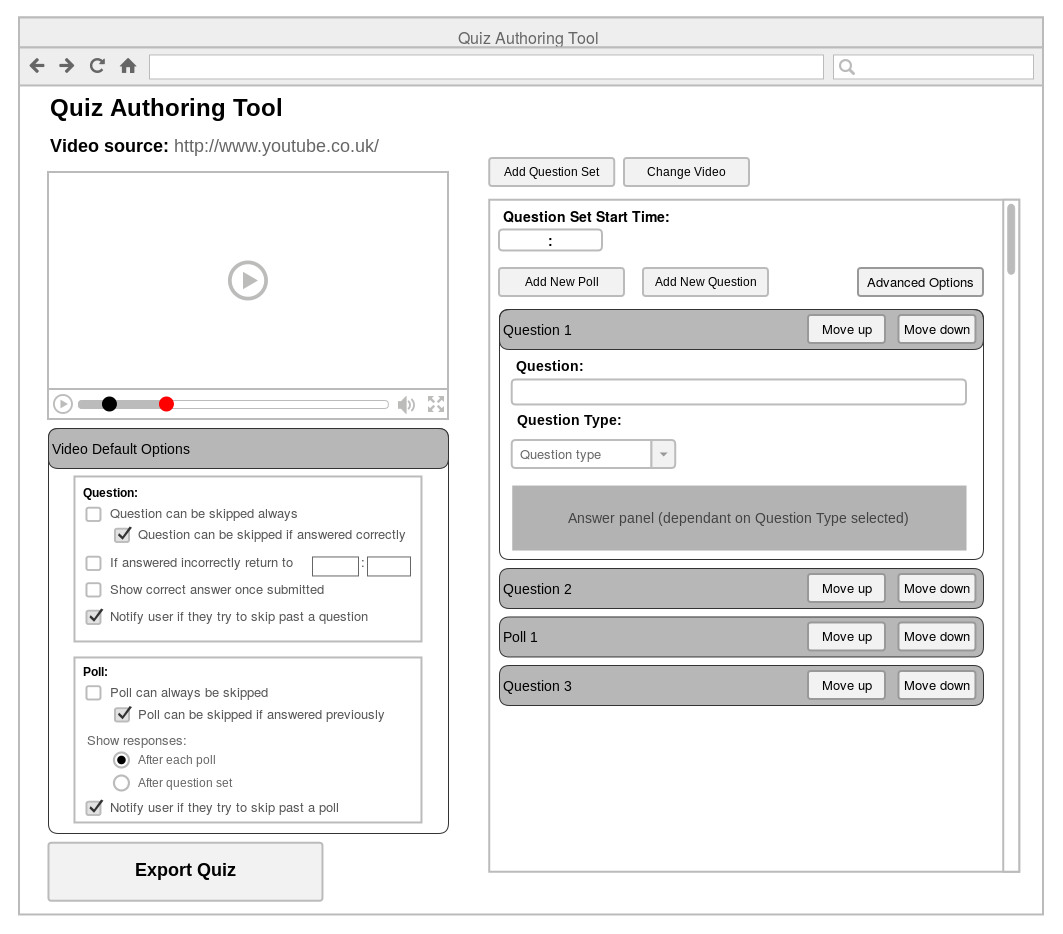
\includegraphics[width=\textwidth]{wireframes/gdpAuthoringAccordianVideoDefaultOptions.png}
	\caption{Wireframe showing the accordion type design of showing/hiding options}
	\label{Figure:wireframes/authoringtool/accordion}
\end{figure}

\subsection{Second Option - Popups}

We considered a second option where you would press an edit button and the options would pop up. Here you originally see the main screen shown in \autoref{Figure:wireframes/authoringtool/main} and then once you select an options button such as the ``advanced option'' button, you would see the popup shown in \autoref{Figure:wireframes/authoringtool/mainPopup}.

\begin{landscape}

\begin{figure}
	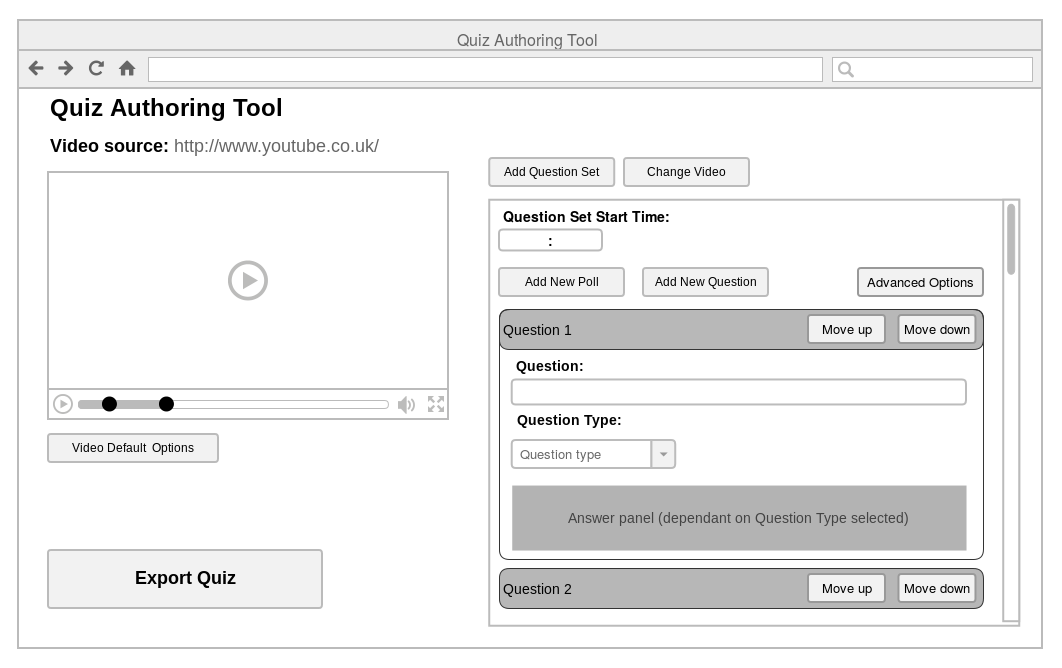
\includegraphics[width=22cm]{wireframes/gdpAuthoringMain.png}
	\caption{Wireframe showing the pop type design of showing/hiding options before opening a popup.}
	\label{Figure:wireframes/authoringtool/main}
\end{figure}

\begin{figure}
	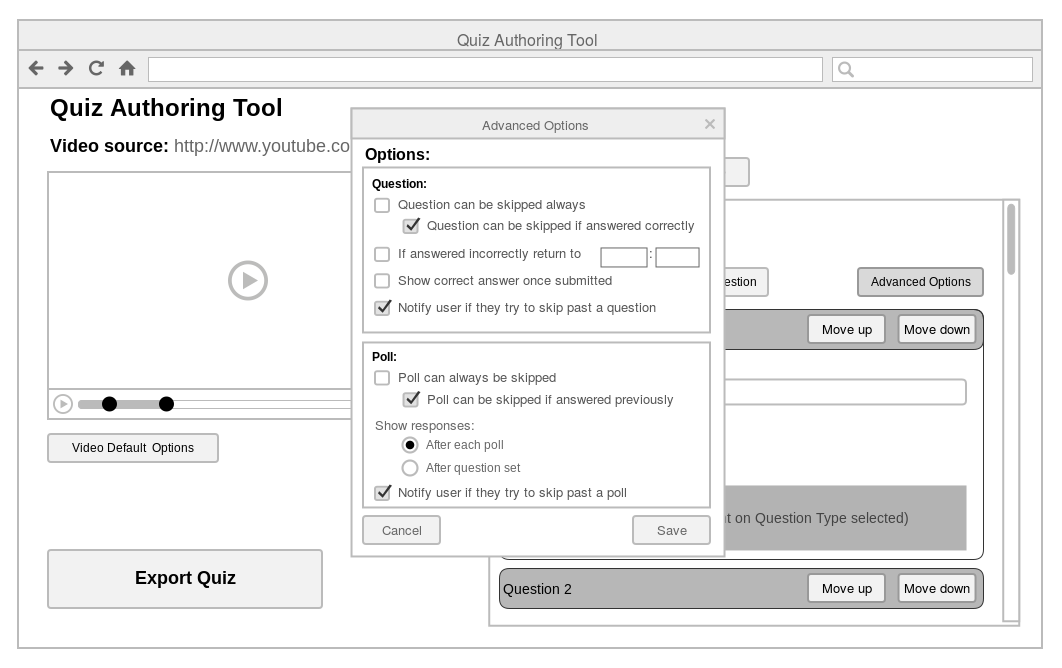
\includegraphics[width=22cm]{wireframes/gdpAuthoringAdvancedOptions.png}
	\caption{Wireframe showing the accordion type design of showing/hiding options after opening a popup.}
	\label{Figure:wireframes/authoringtool/mainPopup}
\end{figure}
\end{landscape}


\section{Question Creation wireframes}

These first wireframes (\autoref{Figure:wireframes/authoringtool/singlePoll}, \autoref{Figure:wireframes/authoringtool/singleQuiz}, \autoref{Figure:wireframes/authoringtool/multiPoll}, \autoref{Figure:wireframes/authoringtool/multiQuiz}, \autoref{Figure:wireframes/authoringtool/rangeStarPoll}, \autoref{Figure:wireframes/authoringtool/rangeStarQuiz}) show how the questions were originally planned to look. This demonstrates the differences between the poll and quiz type options, where the quiz type questions allow the choice of a "correct" answer. These were used to generate the first iteration of HTML mockups, once we had the mockups we used the HTML and iterated over them. This was because it was easier to have more realistic models to present to users and the client.

\begin{figure}
	\centering
	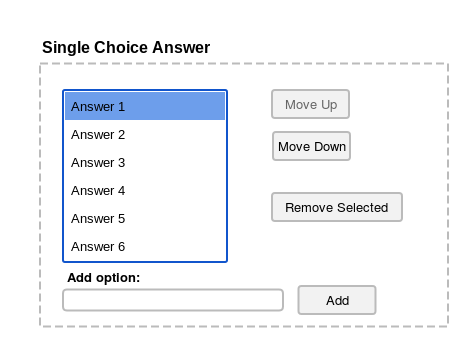
\includegraphics[width=12cm]{wireframes/gdpauthoringsingleanswerpoll.png}
	\caption{A wireframe showing the possible interface when creating a single choice poll type question}
	\label{Figure:wireframes/authoringtool/singlePoll}
\end{figure}

\begin{figure}
	\centering
	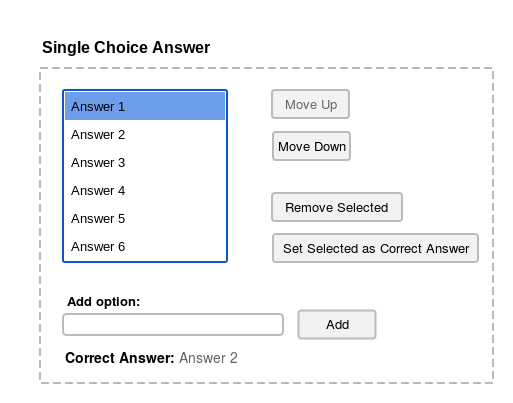
\includegraphics[width=12cm]{wireframes/gdpauthoringsingleanswerquestion.png}
	\caption{A wireframe showing the possible interface when creating a single choice quiz type question}
	\label{Figure:wireframes/authoringtool/singleQuiz}
\end{figure}

\begin{figure}
	\centering
	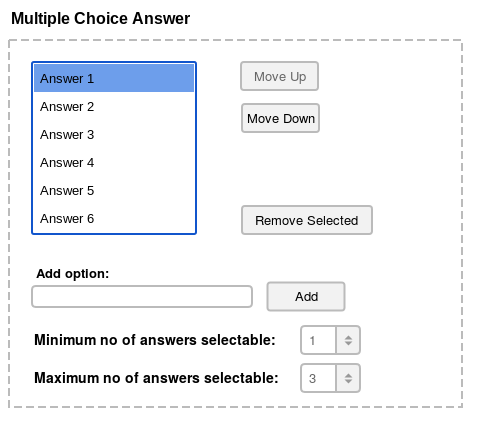
\includegraphics[width=10cm]{wireframes/gdpauthoringmultianswerpoll.png}
	\caption{A wireframe showing the possible interface when creating a multiple choice poll type question}
	\label{Figure:wireframes/authoringtool/multiPoll}
\end{figure}

\begin{figure}
	\centering
	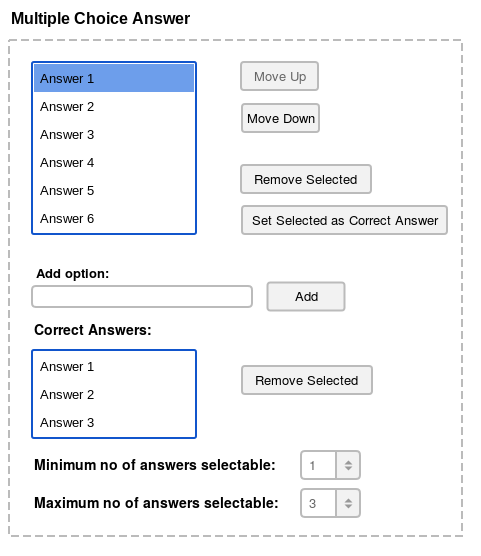
\includegraphics[width=10cm]{wireframes/gdpauthoringmultianswerquestion.png}
	\caption{A wireframe showing the possible interface when creating a multiple choice quiz type question}
	\label{Figure:wireframes/authoringtool/multiQuiz}
\end{figure}

\begin{figure}
	\centering
	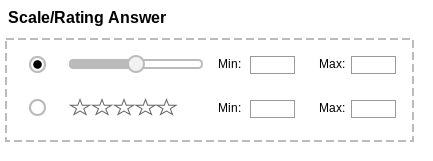
\includegraphics[width=10cm]{wireframes/gdpauthoringscalepoll.png}
	\caption{A wireframe showing the possible interface when creating a range or star poll type question}
	\label{Figure:wireframes/authoringtool/rangeStarPoll}
\end{figure}


\begin{figure}
	\centering
	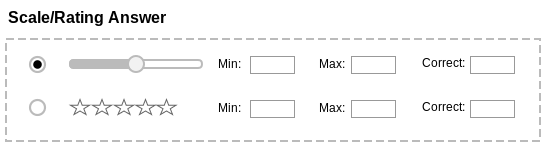
\includegraphics[width=12cm]{wireframes/gdpauthoringscalequestion.png}
	\caption{A wireframe showing the possible interface when creating a range or star quiz type question}
	\label{Figure:wireframes/authoringtool/rangeStarQuiz}
\end{figure}

\section{Accessibility Tooltips}

To aid accessibility we have planned to make tooltips appear on elements. This was illustrated in the example tooltip wireframe \autoref{Figure:wireframes/authoringtool/tooltip}.

\begin{landscape}
\begin{figure}
	\centering
	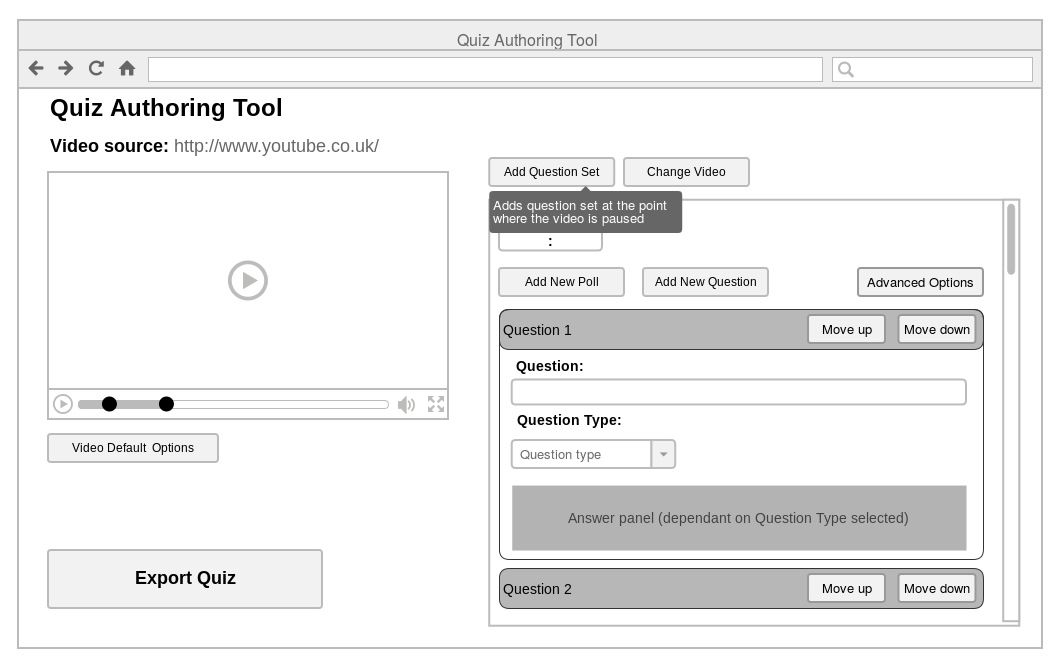
\includegraphics[width=22cm]{wireframes/gdpAuthoringToolTip.png}
	\caption{A wireframe showing an example of how tooltips could be implemented}
	\label{Figure:wireframes/authoringtool/tooltip}
\end{figure}
\end{landscape}

\chapter{Minutes of Meetings} \label{Chapter:Minutes of Meetings}

This appendix contains the minutes of meetings held with the group's supervisor, client and second examiner, as recorded by Harry Cutts. It also contains minutes for our Sprint Retrospectives, where there were any.

Unless otherwise stated, all five group members attended all meetings. Mike Wald attended all client/supervisor meetings as both client and supervisor.

\section{29th September 2014}\label{Minutes:2014-09-29}

\subsection{Client/supervisor meeting}

Yunjia Li (lead developer on Synote) also attended.

\subsubsection{History of Synote}

Mike Wald started by giving a brief history of Synote.

The 2008 version (which is the version running on \texttt{synote.org})
was built with Google Web Toolkit and Grails.

The 2010 version replaced the front-end, but re-used the back-end. A
mobile interface was later added to this version.

A version for the Raspberry Pi was produced.

The new version of Synote is to be built with a node.js back-end, which
will interact with an AngularJS front-end via a ReST API. The code is to
be hosted on GitHub.

\subsubsection{Our task}

Our task is to work on software for interactive video quizzes to be
integrated with Synote at a later date. The solution must be accessible.
We may wish to use the QTI standard for defining quizzes.

This has been done before by a Masters student called Nadia, but her
work was not compatible with AngularJS. Mike will send Nadia's
implementation and report to us. There is also an existing AngularJS
library for interactive video quizzes, which we could fork.

Other requirements:

\begin{itemize}
\itemsep1pt\parskip0pt\parsep0pt
\item
  Use ReSTful APIs to connect the front-end and back-end
\item
  Define a data structure which we can statically serve for the proof of
  concept
\item
  Consider mobile browsers
\item
  Make proper tests
\item
  We'll need to choose a framework
\item
  Later in the project, create a quiz authoring tool
\end{itemize}

The project should be managed in an Agile way. Harry suggested that we
follow SCRUM. Yunjia recommended the RallyDev application for issue
management.

We will hold these meetings with Mike regularly at 14:00 on Mondays. The
group will meet after the GDP briefing on Wednesday.

\subsection{After-meeting}

Sam suggests that we create a very basic prototype and then ask whether
this is what they want.

Harry suggested not scheduling anything over Christmas.

We should find some users and talk to them

SCRUM (with 1 week sprints) would be good to try.

We each should:

\begin{itemize}
\itemsep1pt\parskip0pt\parsep0pt
\item
  Read Nadia's report
\item
  Have a look at the AngularJS Video Quiz module (Chris will email us the link)
\end{itemize}

Harry will create the Google Drive folder, upload the minutes, create a
GitHub organisation and add everyone in the group.

\section{6th October 2014}\label{Minutes:2014-10-06}

\subsection{Client/supervisor meeting}

Shameem Bajar, a third-year student of Information Technology in
Organisations, also attended.

We presented a prototype system built on Videogular over the last week.

Videogular Quiz wasn't worth building on.

Shameem is doing a third-year project, and will be interacting with
users.

Aspects which we haven't covered in our prototype:

\begin{itemize}
\itemsep1pt\parskip0pt\parsep0pt
\item
  Jumping back to sections when questions are answered incorrectly
\item
  Analytics on user behaviour around the quiz
\end{itemize}

A big use case for this project is for the live version. Another is for
MOOCs.

Our technical goals are to overlay quiz questions and polls over online
videos, with analytics support.

Over the next week, we will:

\begin{itemize}
\itemsep1pt\parskip0pt\parsep0pt
\item
  write the brief (sending a draft to Mike),
\item
  make the prototype code more robust, and
\item
  test the prototype on multiple platforms, building up a list of
  issues.
\end{itemize}

As soon as possible, we will get a demo working which can be used by
Shameem to get user feedback and stories.

\subsection{After-meeting}

We could draw some state machines of possible quizzes.

Some questions for us to answer:

\begin{itemize}
\itemsep1pt\parskip0pt\parsep0pt
\item
  Would MediaElement.js be worth investigating?
\item
  Is Videogular's accessibility up to Mike's standards?
\end{itemize}

\section{13th October 2014}\label{Minutes:2014-10-13}

\subsection{Client/supervisor meeting}

We demonstrated our progress on the prototype, including it running on a
phone and a tablet. Mike reiterated that the user should be able to jump
back in the video when a question is answered incorrectly.

We asked how we are to acquire realistic data with which to test the
analytics system. Mike rejected our selection of him using a prototype
system for a lecture, but suggested that Shameem could use focus groups
to acquire data.

He also clarified that the actual analysis of the data is basically as a
proof-of-concept. The important part is to have the front-end collect
the data (in the form of event logs).

We attempted to demonstrate some accessibility improvements which we
have made and contributed to Videogular, but they had not yet been
deployed on the demonstration machine.

We asked whether we could access the code for the new version of Synote,
and learned that Yunjia hasn't started on the new Synote yet.

\section{20th October 2014}\label{Minutes:2014-10-20}

\subsection{Client/supervisor meeting}

We demonstrated:

\begin{itemize}
\itemsep1pt\parskip0pt\parsep0pt
\item
  Videogular accessibility improvements
\item
  Skipping back in the video when a wrong answer is given
\item
  The new stars question type
\end{itemize}

We explained the architecture on which we had decided for the questions
front-end, in which a WebWorker (a sandboxed JavaScript thread) is used
to execute potentially unsafe quiz definitions. This allows us to use
JavaScript to define quizzes in a flexible manner without a complicated
markup language.

Mike said he would think about organising a focus group to collect data
from.

We reported on our first sprint of the project.

We said we would prepare a stable demo for Wednesday, and give the link
to Shameem for user feedback.

\subsubsection{The presentation}

We discussed how to pitch the idea of our project in the up-coming
progress presentation.

Chris Hewett suggested we `sell' the idea of teaching in small chunks
and testing on each individual chunk. Small chucks can be revisited
easily, but splitting a video into those small chunks is very
time-consuming. Instead, our project will allow questions to be inserted
at the end of each chunk in a longer video.

\subsection{Sprint retrospective}

In the traditional SCRUM way, we discussed how well our first sprint had
gone.

\subsubsection{The good}

\begin{itemize}
\itemsep1pt\parskip0pt\parsep0pt
\item
  We got everything that was assigned in the planning meeting done.
\item
  We communicated well.
\end{itemize}

\subsubsection{The bad}

\begin{itemize}
\itemsep1pt\parskip0pt\parsep0pt
\item
  We underestimated the amount of work we could get done.
\item
  Our points allocations were out of whack quite a bit.
\end{itemize}

\section{27th October 2014}\label{Minutes:2014-10-27}

There was no meeting this week as Mike was away.

\subsection{Retrospective}

We didn't all make our points targets this week. This was mostly due to
the presentation.

Poll and Cuepoints issues weren't well defined enough.

Chewett is blocking on lack of documentation and schemas when creating
examples. We should create issues to finalise schemas.

\section{10th November 2014}\label{Minutes:2014-11-10}

\subsection{Client/supervisor meeting}

Yunjia Li and Shameem Bajar also attended.

We demonstrated:

\begin{itemize}
\itemsep1pt\parskip0pt\parsep0pt
\item
  Charts showing results of in-video polls.
\item
  The heat map plug-in for Videogular.
\item
  Our Videogular Analytics plug-in acquiring analytics data, and it
  being processed into a heat map.
\end{itemize}

We mentioned that we need to use HTML5 events (including seek) instead
of watches to detect changes in the video state. We also need to display
the heat map data using the plug-in we've created for Videogular.

Yunjia raised concerns about the perceived difficulty of deploying our
server-side code. We said we would write a document describing the
deployment process to an Apache server.

\subsubsection{Shameem's study}

Shameem presented some initial results of her user studies. The
presentation will be sent to us shortly.

Feedback on the idea was positive. No users mentioned mobile devices,
except that a participant would submit poll responses from a phone
during a lecture (which is out of the scope of our project).

Many suggestions were made by users, some of which were out of scope.
The following were in scope:

\begin{itemize}
\itemsep1pt\parskip0pt\parsep0pt
\item
  Add number of attempts field to authoring tool.
\item
  Give a grade at the end of the quiz.
\item
  Recommend further videos on the same topic after the video is finished
  (which we could display as custom HTML on a results page).
\end{itemize}

We discussed the upcoming presentation, during which we are planning to
demonstrate the analytics view.

\subsection{Retrospective}

\begin{itemize}
\itemsep1pt\parskip0pt\parsep0pt
\item
  We have inconsistency between tabs and spaces for indentation in some
  files.
\item
  Some external libraries are stored inconsistently (e.g.~Bootstrap is a
  submodule in the analytics back-end, d3 is a file in the repository).
\item
  We can use \texttt{bower link} instead of the shell script for using
  Bower with modules which are in development. This will be done in the
  next sprint.
\end{itemize}

\section{17th November 2014}\label{Minutes:2014-11-17}

\subsection{Sprint retrospective}

\begin{itemize}
\itemsep1pt\parskip0pt\parsep0pt
\item
  Number of points per person was good
\end{itemize}

\subsection{Client/supervisor meeting}

We demonstrated the authoring tool UI which has been designed, but not
made functional.

We showed the presentation planned for Wednesday. Mike suggested to
mention the interactive features such as skipping back in the video.

\section{24th November 2014}\label{Minutes:2014-11-24}

\subsection{Meeting with Gary Wills}

\begin{itemize}
\item
  Report is what Gary's going to mark
\item
  UML in design section
\item
  Why didn't we present it to users for evaluation?

  \begin{itemize}
  \itemsep1pt\parskip0pt\parsep0pt
  \item
    The customer (Mike) thinks that it is not viable.
  \end{itemize}
\item
  Write about testing and/or scenario based testing instead.
\item
  Could evaluate based on ``How well does this output suit your
  requirements?''
\item
  Doing team skills audit will improve mark
\item
  Don't include `if we have time' things in goals
\item
  Should have a consistent voice throughout the report
\item
  We \textbf{should not} be working through Christmas
\item
  Manage the customer (Mike)
\item
  ``The key to good assessment is instant feedback.''
\item
  Go through report with fine-tooth spelling and grammar comb before
  submitting report.
\end{itemize}

\subsection{Client/supervisor meeting}

Mike said he was generally happy with our latest progress presentation.

Looking at the authoring tool:

\begin{itemize}
\itemsep1pt\parskip0pt\parsep0pt
\item
  It would be good to make single choice question type a special case of
  multiple choice question.
\item
  A ``Load current time'' button next to the time selector would be
  useful.
\end{itemize}

We should mention that (some) server implementations are example only
and have no scalability guarantees.

\section{1st December 2014}\label{Minutes:2014-12-01}

\subsection{Client/supervisor meeting}

Yunjia Li also attended.

We demonstrated the authoring tool.

Yunjia suggested something for the Further Work report section: making
encoding the video for different browsers/platforms more user-friendly.

Chewett proposed a list of deliverables:

\begin{itemize}
\itemsep1pt\parskip0pt\parsep0pt
\item
  Videogular Questions

  \begin{itemize}
  \itemsep1pt\parskip0pt\parsep0pt
  \item
    Example proof-of-concept site (Videogular Questions Example)
  \end{itemize}
\item
  Videogular Cuepoints

  \begin{itemize}
  \itemsep1pt\parskip0pt\parsep0pt
  \item
    As demonstrated is Videogular Questions Example
  \end{itemize}
\item
  Videogular Heat Maps
\item
  Videogular Analytics

  \begin{itemize}
  \itemsep1pt\parskip0pt\parsep0pt
  \item
    API specification for Videogular Analytics
  \item
    Analytics back-end is an example only
  \end{itemize}
\item
  Authoring tool
\end{itemize}

Mobile browsing will be part of future work.

Mike approved that list of deliverables.

\section{8th December 2014}\label{Minutes:2014-12-08}

\subsection{Client/supervisor meeting}

Yunjia Li also attended.

\subsubsection{Sign off on deliverables}

The deliverables had been sent to Mike last Thursday. He had found that
the heat map did not appear in the analytics interface in Google Chrome.
We clarified a misunderstanding about the vertical scales on results
charts.

Yunjia asked about the status of the seek event in the analytics
plug-in, which has not been implemented but should not be problematic.

Mike and Yunjia said that they were satisfied with the deliverables.
Yunjia said they were `pretty cool'.

Mike said he'd be happy to comment on draft report stuff we send him.

\subsection{After-meeting}

We discussed the report structure, and decided to put all the testing in
one section (with subsections for each component), to emphasize the
range of testing methods we used.

\chapter{Coding Conventions} \label{App:Coding Conventions}

\begin{preamble}
	An appendix detailing the coding conventions and standards for the project.
	\preamblequote{How standards proliferate: \\ Situation: There are 14 competing standards \\ Researcher: 14?! Ridiculous! We need to develop one universal standard that covers everyone's use case! \\ Soon: \\ Situation: There are now 15 competing standards}{XKCD - web comic\footnote{XKCD Standards - \url{http://xkcd.com/927/}}}
\end{preamble}

\section{Introduction}

This appendix contains the coding conventions, from the GitHub repository\footnote{\url{https://github.com/soton-ecs-2014-gdp-12/conventions}}.

\section{General}

File names should be in Unix form (lower-case, words separated by
hyphens, e.g. \texttt{a-directory/my-file.type}).

\section{CSS coding conventions}

Tabs should be used for indentation.

\subsection{Property ordering}

In general, properties further towards the top should affect layout,
while properties towards the bottom should affect appearance.

Specifically, the most common properties should be in this order:

\begin{lstlisting}
.class {
	position
	display

	flex /* etc. */

	top
	bottom
	left
	right
	z-index

	width  /* also min-, max- */
	height /* also min-, max- */

	padding
	border
	margin

	font /* etc. */
	text-align
	background /* etc. */
	color
}
\end{lstlisting}

\section{HTML coding conventions}

All full HTML pages should specify
\texttt{\textless{}!DOCTYPE html\textgreater{}}.

\subsection{Indentation}

Tabs should be used up to the indent level, with spaces for lining up
tags which break over multiple lines.

\subsection{Attributes}

Attribute values should be quoted.

The \texttt{id} attribute should always be first after the tag name,
followed by the \texttt{class} attribute. For meta tags, the
\texttt{name} should be specified first.

\subsection{Scripts}

Where possible, scripts should be imported at the end of the body. For
JavaScript files, the optional \texttt{type} attribute should be
omitted.

\section{Issue tracker usage guidelines}

If an issue doesn't seem to fit with any particular repository, file it
against the \gls{vgQuestions} repository.

The issue type should be described with a label (one of bug,
enhancement, or investigate).

\subsection{waffle.io and Sprint management}

There is a waffle.io board\footnote{\url{https://waffle.io/soton-ecs-2014-gdp-12/videogular-questions/}}
for tracking the Sprints.

Each Sprint will have a milestone on each repository, named ``Sprint '',
with the due date set to that of the Sprint Retrospective meeting. When
an issue is added to a Sprint, it should be added to that Sprint's
milestone.

\section{JavaScript coding
conventions}

Strict mode should be used (\lstinline|`use strict';|). Semicolons should
never be omitted.

In object definitions, trailing commas should always be used. For
example:

\begin{lstlisting}[language=javascript]
obj = {
    foo: 'bar',
    baz: 'quux',
}
\end{lstlisting}

\subsection{Indentation}

Indentation should be done with tabs up to the indent level, and then
spaces for lining up multi-line statements. For example (where a
\texttt{\textgreater{}} is a tab and a \texttt{.} is a space):

\begin{lstlisting}[language=javascript]
function foo() {
>   if (bar === 4) {
>   >   baz("Some really ridiculously long string that should be "
>   >   ....+ "avoided, even mentioned in the coding conventions.");
>   }
}
\end{lstlisting}

This allows other developers to choose indent sizes without messing up
neatly lined-up parts.

\subsection{Naming}

Names should be camel case. The first letter should be lower-case,
except for class names or constructors:

\begin{lstlisting}[language=javascript]
LightBulb = (function() {
    function LightBulb() {
        // ...
    }

    return LightBulb;
})();

var numberOfEngineers = 5;
function changeLightBulb(bulb) {
    // ...
}
\end{lstlisting}

File names should still be in Unix form (e.g. \texttt{light-bulb.js}).
Unit test files should have the same name as the file which they test,
followed by \texttt{\_test} (e.g. \texttt{light-bulb\_test.js}).

\subsection{Types}

The section of JavaScript Garden on Types
\footnote{\url{https://bonsaiden.github.io/JavaScript-Garden/\#types}}
gives a number of guidelines (in the conclusion paragraphs) which should
be followed.

\subsection{JSHint}

JSHint directive comments should be kept to a minimum, with
configuration moved into the \texttt{.jshintrc} file where possible. If
file-specific configuration is necessary, it should go at the top of the
file (before \lstinline|`use strict';|) unless:

\begin{itemize}
\item
  it is specific to a section of the file, or
\item
  it describes the changes made to the environment by a particular line
  of code, for example by the \texttt{importScripts} method in a \gls{webworker}. In this case the directive should be on the next line,
  indented. For example:

\begin{lstlisting}[language=javascript]
importScripts("../../app/bower_components/videogular-questions/questions-worker.js");
    /* global loadAnnotations */
\end{lstlisting}
\end{itemize}

\subsection{AngularJS}

\subsubsection{Dependency injection}

When defining a directive, service, view, controller, etc., and
dynamically injecting dependencies, make sure to pass the parameter name
as a string into the array. For example:

\begin{lstlisting}[language=javascript]
angular.module("com.example.foobar", [])
    .directive(
    "ngFooBar",
    ["$window", "VG_STATES", function($window, VG_STATES) {
        ...
    }])
\end{lstlisting}

This stops minifiers from breaking the dependency information when they
rename parameters.

\section{LaTeX}

\subsection{TODOs}

For todo notes, use the \texttt{\textbackslash{}todo} command. For
example:

\begin{lstlisting}[language=tex]
\todo{Discuss farming in the Middle East.}
\end{lstlisting}

\subsection{References}

When making references, use \texttt{autoref}, like so:

\begin{lstlisting}[language=tex]
\autoref{my-label}
\end{lstlisting}

\subsection{Labelling scheme}

Figure labels should begin with \texttt{Figure:}, chapter labels with
\texttt{Chapter:}, and section labels with \texttt{Section:}.

\section{Python coding conventions}

PEP8 \footnote{\url{http://legacy.python.org/dev/peps/pep-0008/}} should be
followed.

\subsection{File names}

File names should be python style, that is, words separated by
underscores (e.g. \texttt{voluminous\_octopus.py}).

When a virtual environment is used, it should be called \texttt{venv}.
Any dependencies should be defined in \texttt{requirements.txt}.

%TC:endignore

\end{document}
%% ----------------------------------------------------------------
